\documentclass{IEEEoj}
\usepackage[T1]{fontenc}
\let\labelindent\relax
\usepackage{amsmath,amssymb,amsthm,booktabs,longtable,array,graphicx,xcolor,tikz,enumitem}

\usepackage{placeins}
\usepackage[colorlinks=true,linkcolor=blue,citecolor=blue,urlcolor=blue]{hyperref}
\usetikzlibrary{arrows.meta,positioning,calc}
\setlength{\parskip}{0pt}
\setlength{\emergencystretch}{3em}
\renewcommand{\topfraction}{0.94}\renewcommand{\dbltopfraction}{0.95}\renewcommand{\dblfloatpagefraction}{0.8}\setcounter{dbltopnumber}{3}
\renewcommand{\bottomfraction}{0.9}
\renewcommand{\textfraction}{0.04}
\renewcommand{\floatpagefraction}{0.85}
\setlist{nosep,leftmargin=*}
\renewcommand{\arraystretch}{1.15}
\newtheorem{proposition}{Proposition}
\newcommand{\pos}[1]{\left[#1\right]^+}
\newcommand{\norm}[1]{\left\lVert#1\right\rVert_1}
\newcommand{\algline}[3]{\node[anchor=west,align=left,text width=\dimexpr\linewidth-#2cm-25pt\relax,font=\fontsize{8.5}{10}\selectfont,text=black,inner xsep=2pt] at (#2,-.48*#1) {#3};\node[anchor=east,font=\scriptsize\sffamily,text=black!55] at (-.17,-.48*#1) {#1}}

\title{Reliability-Screened Capacity Elasticity under Delayed Telemetry and Actuation: An O-RAN-Motivated Study}
\author{FATIMA SUBHI KHALEEL\textsuperscript{1}, YASSIR AL-AMEEN\textsuperscript{1}, AND HAMED AL-RAWESHIDY\textsuperscript{2}}
\affil{Department of Communications Engineering, College of Engineering, University of Diyala, Baqubah, Iraq (e-mail: fatima.subhi\_eng@uodiyala.edu.iq).}
\affil{College of Engineering, Design and Physical Sciences, Brunel University of London, Uxbridge, U.K.}
\corresp{CORRESPONDING AUTHOR: HAMED AL-RAWESHIDY (e-mail: hamed.al-raweshidy@brunel.ac.uk).}
\AtBeginDocument{\definecolor{ojcolor}{cmyk}{0.93,0.59,0.15,0.02}}
\def\OJlogo{\parbox{125pt}{\sffamily\bfseries\fontsize{7}{8}\selectfont\color{ojcolor}IEEE OPEN JOURNAL OF THE\\COMMUNICATIONS SOCIETY}}
\markboth{Reliability-Screened Capacity Elasticity}{Khaleel et al.}
% Submission copy: no assigned DOI, volume, acceptance date or copyright claim.
\usepackage{etoolbox}
\makeatletter
\patchcmd{\@maketitle}{\receivedfont}{\receivedfont\iffalse}{}{}
\patchcmd{\@maketitle}{\@editor\fi\par}{\@editor\fi\par\fi}{}{}
\def\ps@submission{\def\@oddhead{\hfill\OJlogo}\let\@evenhead\@oddhead\def\@oddfoot{\hfil\rffont Submission manuscript\hfil\thepage}\let\@evenfoot\@oddfoot}
\makeatother
\date{}

\definecolor{ink}{HTML}{243B53}
\definecolor{signal}{HTML}{087F8C}
\definecolor{command}{HTML}{D87525}
\definecolor{pale}{HTML}{EEF4F8}
\tikzset{
 pics/radio/.style={code={
  \draw[ink,line width=1.2pt] (0,.5)--(-.34,-.52)--(.34,-.52)--cycle;
  \draw[ink,line width=.8pt] (-.19,-.08)--(.19,-.08) (-.27,-.32)--(.27,-.32);
  \fill[signal] (0,.57) circle (.065);
  \draw[signal,line width=1pt] (-.22,.38) arc[start angle=220,end angle=140,radius=.29]
   (.22,.38) arc[start angle=-40,end angle=40,radius=.29];
  \draw[signal,line width=1pt] (-.42,.23) arc[start angle=220,end angle=140,radius=.54]
   (.42,.23) arc[start angle=-40,end angle=40,radius=.54];
  \draw[ink,line width=.8pt,rounded corners=1pt] (-.94,-.48) rectangle (-.65,.05);
  \draw[signal,line width=.7pt] (-.89,-.34)--(-.70,-.34);
 }},
 pics/router/.style={code={
  \path[fill=pale,draw=ink,line width=1pt] (-.7,-.27)--(.5,-.27)--(.76,-.04)--(-.44,-.04)--cycle;
  \path[fill=white,draw=ink,line width=1pt] (-.7,-.27)--(.5,-.27)--(.5,-.60)--(-.7,-.60)--cycle;
  \path[fill=ink!12,draw=ink,line width=1pt] (.5,-.27)--(.76,-.04)--(.76,-.37)--(.5,-.60)--cycle;
  \foreach \x in {-.53,-.31,-.09,.13}{\draw[ink,line width=.65pt] (\x,-.36) rectangle +(0.13,-.12);}
  \draw[signal,->,line width=1pt] (-.15,.14)--(-.65,.14);
  \draw[signal,->,line width=1pt] (.15,.34)--(.65,.34);
  \draw[signal,->,line width=1pt] (0,.24)--(0,.72);
 }},
 pics/server/.style={code={
  \path[fill=ink!10,draw=ink,line width=.8pt] (.43,-.65)--(.67,-.47)--(.67,.61)--(.43,.43)--cycle;
  \path[fill=pale,draw=ink,line width=.8pt] (-.48,.43)--(-.24,.61)--(.67,.61)--(.43,.43)--cycle;
  \foreach \y in {-.48,-.1,.28}{
   \path[fill=white,draw=ink,rounded corners=1pt,line width=.9pt] (-.48,\y-.17) rectangle (.43,\y+.17);
   \fill[signal] (-.32,\y) circle (.045);
   \draw[ink!55,line width=.7pt] (-.15,\y)--(.26,\y);
  }
 }},
 pics/control/.style={code={
  \path[fill=white,draw=ink,line width=1pt,rounded corners=2pt] (-.65,-.3) rectangle (.65,.5);
  \draw[ink,line width=1pt] (0,-.3)--(0,-.55) (-.32,-.55)--(.32,-.55);
  \draw[signal,line width=1.1pt] (-.46,-.05)--(-.22,.18)--(.02,.06)--(.23,.32)--(.43,.22);
  \foreach \x/\y in {-.46/-.05,-.22/.18,.02/.06,.23/.32,.43/.22}{\fill[signal] (\x,\y) circle (.035);}
 }},
 pics/report/.style={code={
  \path[fill=white,draw=ink,line width=.9pt,rounded corners=1pt] (-.43,-.57) rectangle (.43,.57);
  \draw[ink!40,line width=.8pt] (-.26,.32)--(.22,.32) (-.26,.15)--(.08,.15);
  \fill[signal!40] (-.26,-.37) rectangle (-.14,-.11);
  \fill[signal!65] (-.04,-.37) rectangle (.08,-.02);
  \fill[signal] (.18,-.37) rectangle (.30,.16);
 }},
 pics/memory/.style={code={
  \foreach \y in {-.37,0,.37}{
   \path[fill=white,draw=ink,line width=.9pt,rounded corners=1pt] (-.57,\y-.13) rectangle (.57,\y+.13);
   \fill[command] (-.39,\y) circle (.04);
   \draw[ink!50,line width=.7pt] (-.21,\y)--(.37,\y);
  }
 }},
 pics/clock/.style={code={
  \draw[command,line width=1pt,fill=white] (0,0) circle (.4);
  \draw[command,line width=1pt] (0,.26)--(0,0)--(.19,-.12);
 }}
}

\begin{document}
\begin{abstract}
Resource elasticity under delayed telemetry can reduce provisioning cost while increasing deadline violations. This study examines that trade-off in an Open Radio Access Network (O-RAN)-motivated, three-stage service chain. A causal controller projects reported queues using applied actions and pending commands, then selects capacity and class reservations on a finite grid. A headroom parameter is calibrated separately under a common classwise mean-miss target of 0.1\%. The experiment comprises 336 calibration and 840 held-out executions across seven settings, with twenty independent test seeds per setting. Comparisons include fixed capacity, target-utilization sizing, a queue-weighted cost controller and component ablations. Three fixed-reference comparisons satisfy the complete descriptive reliability screen and reduce mean incremental cost by 35.61--37.73\%. Markov-modulated traffic, compound arrivals and fifty-slot actuation expose failures of the selected policy. Derived sensitivity relations explain how headroom and demand uncertainty affect surrogate feasibility, while paired intervals quantify observed cost differences. The results establish conditional advantages within a synthetic packet-service model. They do not certify rare-event reliability or validate a physical O-RAN implementation.
\end{abstract}
\begin{IEEEkeywords} O-RAN, software-defined networking, delayed actuation,
telemetry, reliability screening, resource elasticity, reproducible simulation.
\end{IEEEkeywords}
\maketitle
\pagestyle{submission}\thispagestyle{submission}\raggedbottom


\section{Introduction}
An elastic resource controller acts on two different timelines. Its queue report
describes a past state, whereas its next command changes a future service
opportunity. Between those instants, earlier commands can already have altered
capacity. Open Radio Access Network (O-RAN) exposes programmable control across
disaggregated components \cite{polese}. Software-defined networking (SDN)
separates control from forwarding \cite{sdn}, and virtualization makes resource
provisioning an explicit orchestration decision \cite{ecosystem}. These features
motivate accounting for the gap between observing, requesting and activating
resources. They do not make those three events simultaneous.

The resulting ambiguity is operationally important. A controller extrapolating
an old service rate may request capacity that is already scheduled to arrive.
Conversely, a controller that assumes immediate activation may underestimate
the workload accumulated before its command becomes effective. Information-age
analysis characterizes observation freshness \cite{age}, networked control
incorporates delayed feedback \cite{networked}, and predictive control uses
models of future action effects \cite{mpc}. The unresolved question for the
present experiment is narrower: how much does explicitly retaining the known
action history contribute to the cost--deadline trade-off of an otherwise
simple allocator?

That question requires a reliability-aware comparison. Reducing active capacity
almost automatically reduces a capacity-based cost, but can also increase
deadline misses. A lower cost alone is therefore not evidence of a better
allocator. The experiment separates three objects: the stochastic design
objective, the finite-grid proxy used to issue commands, and the empirical
screen used to interpret measured outcomes. This separation prevents a
surrogate-feasible decision or a favorable average cost from being mistaken
for a packet-level guarantee.

The study considers two packet classes traversing three serial service stages,
motivated by access, transport and compute domains. The controller receives
one delayed stage report per control epoch, projects workloads through already
applied and pending commands, and chooses expansion and class reservations.
A headroom parameter is selected on calibration seeds and locked before
testing. All stages use abstract packet-service units. Physical radio channels,
processor execution times and O-RAN interface interoperability are outside
the implemented model.

Three research questions organize the analysis. First, can the calibrated
controller reduce cost against a preprovisioned reference while both pass the
same classwise reliability screen? Second, is the ledger useful at fixed
headroom, and how much of its cost difference comes from capacity versus
switching? Third, do shifted arrival patterns, bottleneck location and command
delay reveal a gap between proxy feasibility and measured deadline risk?

The contributions are an executable action-ledger controller, an explicit
calibration-and-comparison protocol, and a reproducible account of its useful
and failing regimes. The mathematical analysis connects exact age-resolved service, delayed
command activation and deadline-capacity limits to the implemented approximation.
Integer reservation and sensitivity relations explain its ranking rule. The numerical
analysis covers 336 calibration and 840 held-out executions, with matched
traces, component ablations and seed-level uncertainty. Additional diagnostic
decompositions use these saved executions without changing parameter selection
or the original qualification rule. The contribution is this controlled
combination, not a new prediction paradigm, a solution to the full stochastic
control problem, or demonstrated superiority over deployed O-RAN systems.

The remainder develops the literature-based comparison boundary, the service
and information model, the controller and its analytical limits, and the
experimental evidence. Successful comparisons and counterexamples receive
separate treatment before the deployment limitations are discussed.


\section{Related Work and Comparison Boundary}

OrchestRAN chooses intelligence algorithms and their execution locations
\cite{orchestr}, while quality-driven intelligence orchestration deploys and shares near-real-time control
applications (xApps) across network services \cite{oreo}. Their decision objects
are not the packet-stage capacities used here. Joint cloud, fronthaul and radio
orchestration already treats cross-domain resource coupling \cite{demir}.
Consequently, neither a three-domain drawing nor joint resource selection is
the novelty of the present study. The relevant distinction is explicit replay
of already issued commands when stale queue measurements are projected.

Implemented virtualized radio access network (vRAN) systems provide a stronger
physical basis than homogeneous queues. vrAIn learns radio/computing allocation
\cite{vrain}, Nuberu restructures processing under compute deficits
\cite{nuberu}, and Concordia schedules shared computing against processing
deadlines \cite{concordia}. Online-learning base-station allocation
\cite{kalntis} and delay-aware multi-timescale orchestration
\cite{marea} further constrain the novelty claim: adaptation and delay-aware
allocation are established approaches. Proactive workload orchestration
\cite{caora} and learned functional-split selection \cite{murti} also address
anticipation and reconfiguration. None of their reported performance numbers
can be compared directly with an abstract service-unit cost.


Radio-intelligence-controller allocation \cite{wang}, multivariate
probabilistic forecasting \cite{kasuluru}, and online-learning energy-aware
allocation \cite{sora} differ in both prediction machinery and objective.
The predictor here holds reported ingress and base capacity constant. Its
added information is the controller's own action history, not a learned model
of future traffic. This permits an inspectable ablation, but leaves uncertainty
from workload evolution unresolved.

Conflict management studies interactions between xApps \cite{comix}. In contrast, this paper
tracks sequential commands from a single controller. Service-enabled sub-slice
isolation \cite{5erasi} and RadioSaber's channel-aware customizable schedulers
\cite{radiosaber} also provide capabilities that quota borrowing does not
establish. EdgeRIC demonstrates control in an implemented low-latency system
\cite{edgeric}. Its evidence motivates examining delay, but does not justify
assigning a measured real-time meaning to the synthetic slot used below.


ColO-RAN \cite{coloran}, OpenRAN Gym \cite{gym}, a softwarized prototyping platform \cite{scope} and FlexRIC
\cite{flexric} offer programmable experimental foundations. ns-O-RAN
\cite{nsoran}, Colosseum \cite{colosseum} and the fifth-generation (5G) cellular simulator 5G-LENA
\cite{lena}, including its calibration studies \cite{calibration}, identify
possible routes to higher-fidelity validation. These are not platforms executed
in the current study. Listing them does not establish interface compliance.

Queue-based stochastic optimization \cite{neely}, deterministic network calculus
\cite{netcalc} and stochastic network calculus \cite{stochcalc} address distinct
types of guarantees. Analyses of interleaved weighted round-robin \cite{iwrr},
deficit round-robin \cite{drr} and packet-level delay bounds \cite{packetbounds}
depend on precise arrival and service assumptions. The workload score in this
paper is not a service curve, a stability proof or a probabilistic delay bound.
Verification of its implementation is also different from physical validation
of the abstraction \cite{sargent}.

The executed comparator families are deliberately transparent. Kubernetes
Horizontal Pod Autoscaling (HPA) supplies the target-utilization and downscale
stabilization ideas \cite{hpa}. Drift-plus-penalty (DPP) scheduling supplies the
queue-weighted resource-cost trade-off \cite{dppenergy}. Both implementations
below are adaptations, with changed metrics and timing, rather than reproductions
of the original systems or their guarantees. Delay-Tolerant Constrained Online
Convex Optimization (DTC-OCO) studies delayed feedback with constraint and regret
analysis \cite{dtc}. Delayed activation of immutable integer commands is a
different decision setting, so DTC-OCO is positioning literature only.

Table~\ref{tab:related} makes the comparison boundary explicit. The empirical
gap addressed here is the joint accounting of stale reports, known pending
commands and a common reliability screen in a reproducible queue experiment.
It is not a claim that prior systems omit all of these concerns, nor a claim
of state-of-the-art performance without reproducing them.
\begin{table*}[!t]\centering\small
\caption{Study-level comparison of decision scope and evidence. Positioning studies are not executed benchmarks.}
\label{tab:related}
\begin{tabular}{>{\raggedright\arraybackslash}p{23mm}>{\raggedright\arraybackslash}p{43mm}>{\raggedright\arraybackslash}p{47mm}>{\raggedright\arraybackslash}p{47mm}}
\toprule Study & Controlled object and objective & Timing or uncertainty treatment & Relationship to this experiment\\\midrule
\cite{demir} (2024) & Joint cloud, fronthaul and radio resources with an energy objective & Cross-domain resource coupling in cell-free massive multiple-input multiple-output (MIMO) & Joint allocation is established. The present abstract cost is not measured energy.\\
\cite{oreo} (2025) & Placement and sharing of xApp-based services & Quality-driven orchestration of network intelligence & A different decision object from integer packet-stage capacities.\\
\cite{kalntis} (2025) & Resource thresholds balancing vBS performance and energy & Online learning under changing operating conditions & Formal learning analysis does not transfer to the finite-grid workload heuristic here.\\
\cite{marea} (2025) & Radio-resource allocation for delay-sensitive services & Near-real-time latency modeling and real-time queue adaptation & A closer delay-aware reference, but radio-resource and violation models differ. No reproduced performance comparison.\\
\cite{kasuluru} (2026) & Multivariate probabilistic resource-demand forecasts & Learned predictive distributions in a containerized rApp & Forecasting richer future demand differs from replaying known commands with held rates.\\
\cite{sora} (2025) & Energy-efficient O-RAN resource allocation & Online learning & Distinguishes learned adaptation from fixed, separately calibrated headroom.\\
\cite{comix} (2025) & Conflict management across xApps & Interactions between control applications & Here, reordering concerns commands from one controller, not competing xApps.\\
\cite{dtc} (2021) & Constrained online network-resource decisions & Delayed feedback and regret analysis & Feedback delay is distinct from immutable, delayed integer activation.\\
\cite{nuberu,concordia} (2021) & Shared vRAN computation and processing deadlines & Implemented processing and scheduling mechanisms & Stronger physical evidence. No equivalence to the synthetic service chain is asserted.\\
\cite{hpa,dppenergy} & Utilization-based sizing and queue-weighted cost & Stabilization or queue-dependent resource decisions & Adapted comparator families executed on the same traces, grids and delays.\\
Present study & Capacity and class shares under a mean-miss screen & Stale reports, issued-command replay and locked headroom & 336 calibration and 840 held-out executions. Conditional savings and failure regimes, without physical validation.\\
\bottomrule\end{tabular}\end{table*}


\section{System Model and Problem Definition}
The comparison boundary above motivates a model that separates physical packet
evolution from the information available when a command is issued. The following
formulation first specifies service and packet ages, then delayed observations
and actions, and finally the cost and reliability objective.

\subsection{Service chain and scheduling}
Figure~\ref{fig:architecture} identifies the controlled stages and information paths. Table~\ref{tab:notation} summarizes the principal symbols and units.

Let $i\in\{1,2,3\}$ index stages, $s\in\{0,1\}$ index classes and
$t\in\{0,\ldots,T-1\}$ index discrete slots. A packet has a class $s$, birth
slot $b$ and absolute deadline $b+D_s-1$. A packet completed in slot $t$ has
latency $t-b+1$ and is late if that value exceeds $D_s$.
Let $Q_{is}(t)$ denote the queue at the beginning of slot $t$, before external
arrivals, and let $A_s(t)$ denote newly generated packets. Service $S_{is}(t)$
uses total integer capacity $C_i(t)=c_i(t)+e_i(t)$, comprising base capacity
$c_i$ and active paid expansion $e_i$. The implemented dynamics are
\begin{align}
 Q_{1s}(t+1)&=Q_{1s}(t)+A_s(t)-S_{1s}(t),\label{eq:q1}\\
 Q_{is}(t+1)&=Q_{is}(t)-S_{is}(t)+S_{i-1,s}(t),\quad i=2,3.\label{eq:qi}
\end{align}
Stage 1 can serve new arrivals immediately. Stages 2 and 3 serve before their
upstream neighbors, so a packet cannot traverse two stages in one slot.
Each packet requires one service unit at every stage. Class queues are first-in,
first-out (FIFO). There are no drops, retransmissions, alternate routes or
finite-buffer admission decisions.

At each slot the engine applies due commands, delivers due reports, inserts
external arrivals, requests a report and computes a command if the slot is a
control epoch, serves stages in order $3,2,1$, and updates measurement histories.
This ordering fixes otherwise consequential ambiguities at equal timestamps.
Report snapshots are taken after external arrivals and before service.
No new snapshot is visible to the controller before its configured delivery time.

\begin{figure*}[!htbp]\centering
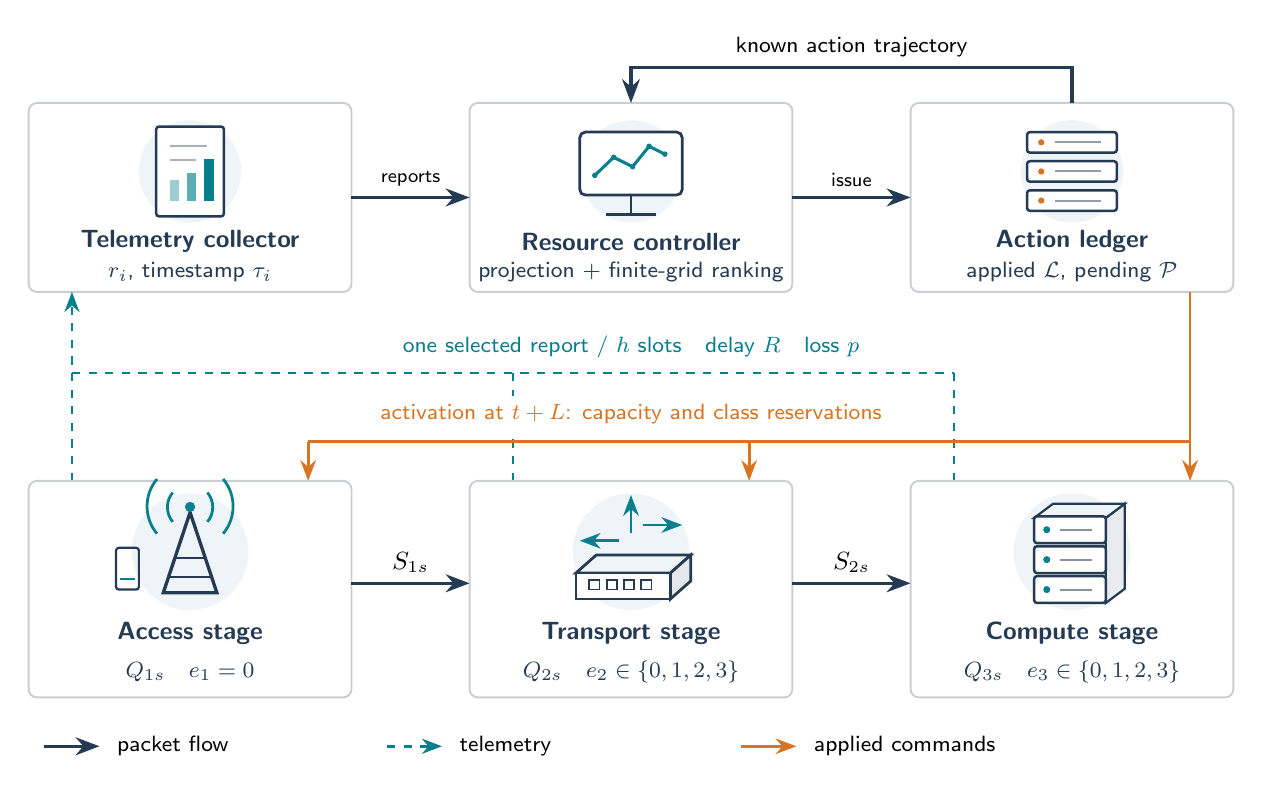
\begin{tikzpicture}[>=Stealth,x=1cm,y=1cm,font=\small\sffamily,
 panel/.style={draw=ink!25,fill=white,rounded corners=3pt,line width=.7pt},
 flow/.style={->,draw=ink,line width=1.25pt},
 telemetry/.style={draw=signal,dashed,line width=.95pt},
 actuation/.style={draw=command,line width=1pt}]
% Controller functions: equipment-inspired icons with explicit model labels.
\foreach \x in {2,7.6,13.2}{
 \path[panel] (\x-2.05,5.15) rectangle (\x+2.05,7.55);
 \path[fill=pale,draw=none] (\x,6.68) circle (.65);
}
\pic at (2,6.68) {report};
\pic at (7.6,6.68) {control};
\pic at (13.2,6.68) {memory};
\node[font=\small\sffamily\bfseries,text=ink] at (2,5.79) {Telemetry collector};
\node[font=\footnotesize\sffamily,text=ink] at (2,5.40) {$r_i$, timestamp $\tau_i$};
\node[font=\small\sffamily\bfseries,text=ink] at (7.6,5.79) {Resource controller};
\node[font=\footnotesize\sffamily,text=ink] at (7.6,5.40) {projection + finite-grid ranking};
\node[font=\small\sffamily\bfseries,text=ink] at (13.2,5.79) {Action ledger};
\node[font=\footnotesize\sffamily,text=ink] at (13.2,5.40) {applied $\mathcal L$, pending $\mathcal P$};
\draw[flow] (4.05,6.35)--node[above,font=\scriptsize\sffamily]{reports}(5.55,6.35);
\draw[flow] (9.65,6.35)--node[above,font=\scriptsize\sffamily]{issue}(11.15,6.35);
\draw[flow] (13.2,7.55)--(13.2,8.0)--node[above,font=\footnotesize\sffamily]{known action trajectory}(7.6,8.0)--(7.6,7.55);
% Separate telemetry and actuation buses prevent crossings through equipment.
\draw[telemetry,->] (.50,2.75)--(.50,5.15);
\draw[telemetry] (.50,4.12)--(11.70,4.12);
\foreach \x in {6.1,11.7}{\draw[telemetry] (\x,2.75)--(\x,4.12);}
\node[text=signal,font=\footnotesize\sffamily,fill=white,inner sep=3pt] at (7.6,4.45)
 {one selected report / $h$ slots\quad delay $R$\quad loss $p$};
\draw[actuation] (14.7,5.15)--(14.7,3.25)--(3.5,3.25);
\foreach \x in {3.5,9.1,14.7}{\draw[actuation,->] (\x,3.25)--(\x,2.75);}
\node[text=command,font=\footnotesize\sffamily,fill=white,inner sep=3pt] at (7.6,3.60)
 {activation at $t+L$: capacity and class reservations};
% Abstract stages are illustrated by familiar access, transport and compute assets.
\foreach \x in {2,7.6,13.2}{
 \path[panel] (\x-2.05,0) rectangle (\x+2.05,2.75);
 \path[fill=pale,draw=none] (\x,1.85) circle (.74);
}
\pic at (2,1.85) {radio};
\pic at (7.6,1.85) {router};
\pic at (13.2,1.85) {server};
\node[font=\small\sffamily\bfseries,text=ink] at (2,.82) {Access stage};
\node[font=\small\sffamily\bfseries,text=ink] at (7.6,.82) {Transport stage};
\node[font=\small\sffamily\bfseries,text=ink] at (13.2,.82) {Compute stage};
\node[font=\footnotesize\sffamily,text=ink] at (2,.32) {$Q_{1s}$\quad $e_1=0$};
\node[font=\footnotesize\sffamily,text=ink] at (7.6,.32) {$Q_{2s}$\quad $e_2\in\{0,1,2,3\}$};
\node[font=\footnotesize\sffamily,text=ink] at (13.2,.32) {$Q_{3s}$\quad $e_3\in\{0,1,2,3\}$};
\draw[flow] (4.05,1.45)--node[above]{$S_{1s}$}(5.55,1.45);
\draw[flow] (9.65,1.45)--node[above]{$S_{2s}$}(11.15,1.45);
\draw[flow] (.15,-.62)--(.85,-.62);
\node[anchor=west,font=\footnotesize\sffamily] at (.95,-.62){packet flow};
\draw[telemetry,->] (4.5,-.62)--(5.2,-.62);
\node[anchor=west,font=\footnotesize\sffamily] at (5.3,-.62){telemetry};
\draw[actuation,->] (9.0,-.62)--(9.7,-.62);
\node[anchor=west,font=\footnotesize\sffamily] at (9.8,-.62){applied commands};
\end{tikzpicture}
\caption{Equipment-inspired view of the three-stage service model and its control loop. Icons identify access, transport and compute roles. They do not imply implemented radio hardware or O-RAN interfaces.}
\label{fig:architecture}\end{figure*}

\begin{table*}[htbp]\centering\footnotesize\renewcommand{\arraystretch}{1.04}
\caption{Notation and units. All capacities and workloads are abstract.}\label{tab:notation}
\begin{tabular}{p{32mm}p{117mm}}\toprule
Symbol & Definition\\\midrule
$Q_{is},A_s,S_{is}$ & Queue, external arrivals and service counts, in packets\\
$c_i,e_i,C_i$ & Base, expansion and total capacity, in packets per slot\\
$D_s,b,T$ & Class deadline, birth slot and run length, in slots\\
$\tau_i,\Delta_i$ & Timestamp of latest delivered stage report and its age $t-\tau_i$\\
$\bar a_{is},\bar\mu_{is},v_{is}$ & Historical mean ingress, mean service and variance of net ingress\\
$h,W,R,L,p$ & Control interval, history window, report delay, activation delay and report loss probability\\
$\alpha,k,\mathcal X$ & Class-0 share, share-grid index and candidate decision set\\
$\mathcal L,\mathcal P$ & Applied-action ledger and pending-command list\\
$\widehat q_{is},d_{is},\rho_s$ & Projected pre-service queue, demand proxy and normalized delay score\\
$\eta,\epsilon,\delta$ & Headroom factor, absolute mean-risk target and paired miss margin\\
$X_{isa},Y_{isa}$ & Age-resolved queued and served packets\\
$m_i,\sigma_{isa},\omega_{sa}$ & Minimum remaining service slots, structural slack and command-relative slack\\
$M_s^{\rm irr}$ & Cohort packets already unable to meet their deadline\\
$J,V_s$ & Full-run incremental cost and cohort deadline-miss fraction\\\bottomrule
\end{tabular}
\end{table*}


For weights $(\alpha,1-\alpha)$, integer reserved service
$g_{is}(C_i,\alpha)$ is obtained by flooring proportional quotas and assigning
the remainder to the largest fractional part, with deterministic class-index
tie breaking. Thus $\sum_s g_{is}=C_i$.
The local scheduler first reserves
\begin{equation}
 \begin{gathered}u_{is}=\min\{B_{is},g_{is}\},\\B_{1s}=Q_{1s}+A_s,\quad B_{is}=Q_{is}\ (i>1).\end{gathered}
\end{equation}
Remaining units are borrowed by the eligible class whose next packet has the
earliest absolute deadline, with class-index ties. This is deadline-based
borrowing after reservations, not unrestricted earliest-deadline-first service.
It ensures $\sum_s S_{is}=\min\{C_i,\sum_s B_{is}\}$.


\subsection{Packet ages and deadline accounting}
Queue length alone does not identify the number of packets approaching their
deadline. Introduce $X_{isa}(t)$, the number of class-$s$ packets at stage $i$
whose age is $a=t-b$, measured after external arrivals and before service in
slot $t$. Let $Y_{isa}(t)$ count the packets of that age served at that stage
in that slot. Both variables are nonnegative integers. This representation
retains the birth timestamps already present in the simulator and does not
add a new measurement to the controller. Its aggregation is
\begin{equation}
\begin{aligned}
 B_{is}(t)&=\sum_{a\ge0}X_{isa}(t),\quad S_{is}(t)=\sum_{a\ge0}Y_{isa}(t),\\
 0&\le Y_{isa}(t)\le X_{isa}(t).
\end{aligned}
\label{eq:ageaggregate}
\end{equation}
Here $B_{1s}=Q_{1s}+A_s$ and $B_{is}=Q_{is}$ for $i>1$, consistent with the
earlier pre-arrival queue convention. With initially empty queues, the exact
age dynamics are
\begin{align}
 X_{1s,0}(t+1)&=A_s(t+1),\nonumber\\X_{is,0}(t+1)&=0\quad(i>1),\label{eq:agebirth}\\
 X_{1s,a+1}(t+1)&=X_{1sa}(t)-Y_{1sa}(t),\label{eq:agefirst}\\
 X_{is,a+1}(t+1)&=X_{isa}(t)-Y_{isa}(t)\nonumber\\&\quad+Y_{i-1,s,a}(t),\quad i=2,3.\label{eq:agetransit}
\end{align}
All survivors age by one slot. Upstream departures become downstream work
for the next slot because service is executed in reverse stage order.
Summing these equations over age recovers the aggregate queue recurrences.
In particular, no packet can traverse two stages in a single slot.

The service constraints combine the stage budget with within-class FIFO:
\begin{align}
 \sum_{s,a}Y_{isa}(t)&=\min\!\left\{C_i(t),\sum_{s,a}X_{isa}(t)\right\},
 \label{eq:agebudget}\\
 Y_{isa}(t)>0&\ \Longrightarrow\
 \sum_{v>a}\bigl[X_{isv}(t)-Y_{isv}(t)\bigr]=0.
 \label{eq:agefifo}
\end{align}
Equation~\eqref{eq:agefifo} requires every older packet of the same class to
be served before a younger age group receives service. Between classes,
reserved quotas and earliest-deadline borrowing still determine the totals
$S_{is}$ through the scheduler already specified. Thus
\eqref{eq:agebudget}--\eqref{eq:agefifo} are necessary service constraints,
not a replacement scheduling optimization with freely selectable departures.
Late packets remain queued and consume service. Truncating all ages at $D_s$
would therefore change the model.

Let $\chi(t,a)=\mathbf1\{b_{\min}\le t-a<b_{\max}\}$ identify the measured
birth cohort, with $b_{\min}=300$ and $b_{\max}=3300$. The indicator
$\mathbf1\{\cdot\}$ is one when its condition holds and zero otherwise.
For $N_s>0$, the deadline-miss fraction has the equivalent exact expression
\begin{equation}
\begin{aligned}
 V_s&=1-\frac1{N_s}\sum_{t=0}^{T-1}\sum_{a=0}^{D_s-1}\chi(t,a)Y_{3sa}(t),\\
 N_s&=\sum_{t=b_{\min}}^{b_{\max}-1}A_s(t).
\end{aligned}
\label{eq:agemiss}
\end{equation}
When $N_s=0$, set $V_s=0$. Completion latency is $a+1$, so the upper limit
$D_s-1$ includes completion exactly at the deadline. Every cohort packet
contributes once to either the on-time count or its complement. The tail
extends beyond all cohort deadlines, making that complement identical to
late completions plus unfinished packets in \eqref{eq:miss}.

This identity also exposes an information loss in the workload proxy. Two
states with the same $B_{is}$ and service reservations can have different
$X_{isa}$ and hence different attainable on-time counts. At the last stage,
one packet of age $D_s-1$ can still finish on time if served immediately,
whereas a packet of age $D_s$ cannot. Their queue lengths are identical.
Aggregate feasibility therefore cannot be sufficient for deadline feasibility
without additional age information or assumptions.

The age state also gives a sharper necessary deadline condition than queue
length alone. A packet at stage $i$ requires at least $m_i=4-i$ further service
slots because adjacent stages cannot serve it in the same slot. Define its
structural slack and the already-unrecoverable measured workload by
\begin{align}
 \sigma_{isa}(t)&=D_s-a-m_i,\label{eq:structuralslack}\\
 M_s^{\rm irr}(t)&=\sum_{i=1}^{3}\sum_{a\ge0}\chi(t,a)X_{isa}(t)
            \mathbf1\{\sigma_{isa}(t)<0\}.\label{eq:hopeless}
\end{align}
Even unlimited capacity cannot recover a packet counted by $M_s^{\rm irr}(t)$ under
the specified event order. Each packet occupies only one stage at that instant.
Consequently, for $N_s>0$,
\begin{equation}
 V_s\ge\frac{\max_{0\le t<T}M_s^{\rm irr}(t)}{N_s}.
 \label{eq:slackbound}
\end{equation}
The maximum, rather than a sum over time, avoids counting the same packet
repeatedly. This is an original necessary condition derived from the age
recurrences, not an imported stochastic delay guarantee. It is not evaluated
as a new empirical metric because the frozen aggregate records do not retain
every $X_{isa}(t)$. Packet-level service assumptions likewise determine the
applicability of established delay bounds \cite{packetbounds,iwrr}.

The currently issued command has an additional timing restriction. Put
$\omega_{sa}(t)=D_s-a-L_t$. When $\omega_{sa}(t)\le0$, the last permissible
completion slot $t+D_s-a-1$ precedes activation at $t+L_t$. Thus the new
command cannot affect that packet's on-time outcome. Earlier active or pending
commands may still serve it successfully. This command-specific restriction
does not imply that all such packets must miss their deadlines.

\subsection{Telemetry, actuation and switching cost}
Every $h=5$ slots, one stage is selected for a report. Its payload is
\begin{equation}
 r_i=(q_i,\bar a_i,\bar\mu_i,v_i,\bar c_i,\tau_i),
\end{equation}
where $q_i$ is the pre-service queue, $\bar c_i$ is the base capacity at the
snapshot, and the rate statistics use the preceding $W=20$ slots.
Specifically, $v_{is}$ is the population variance of stage ingress minus service
over that window. Empty histories use fixed initialization values listed in the
experiment setup. Each request is independently lost with probability $p$ or
delivered after $R$ slots. A report older than the stored timestamp is discarded.

The common risk-based report selector uses
\begin{align}
 \widetilde q_{is}(t)&=\pos{q_{is}+\Delta_i(\bar a_{is}-\bar\mu_{is})},\\
 z_i(t)&=\sum_s\frac{\sqrt{\Delta_i v_{is}+1}}{D_s}
 \left(1+\frac{\widetilde q_{is}(t)}{\max(1,\bar c_i)}\right)+0.01\Delta_i.
\end{align}
The stage with greatest $z_i$ is selected, breaking ties by stage index.
The final age term is a heuristic priority term, not a bounded-starvation proof.
Different methods may select different stages even though their request counts
and request-index loss flags are identical.

Figure~\ref{fig:timeline} relates measurement age, report delivery and command activation. A decision at time $t$ creates an immutable command $(t+L,x,w)$ containing an
expansion vector and stage-wise class weights. All due commands execute. There
is no cancellation, acknowledgment loss or automatic supersession. Constant-delay
runs preserve issuance order. In the variable-delay setting, $L$ is announced
for each issued command, activations may reorder, and commands due in the
same slot execute in issuance order. Future delay draws remain unavailable.
Initial fixed capacity is preprovisioned, whereas elastic methods start with
zero expansion. Fixed methods still update class shares through delayed commands.

\begin{figure*}[!htbp]\centering
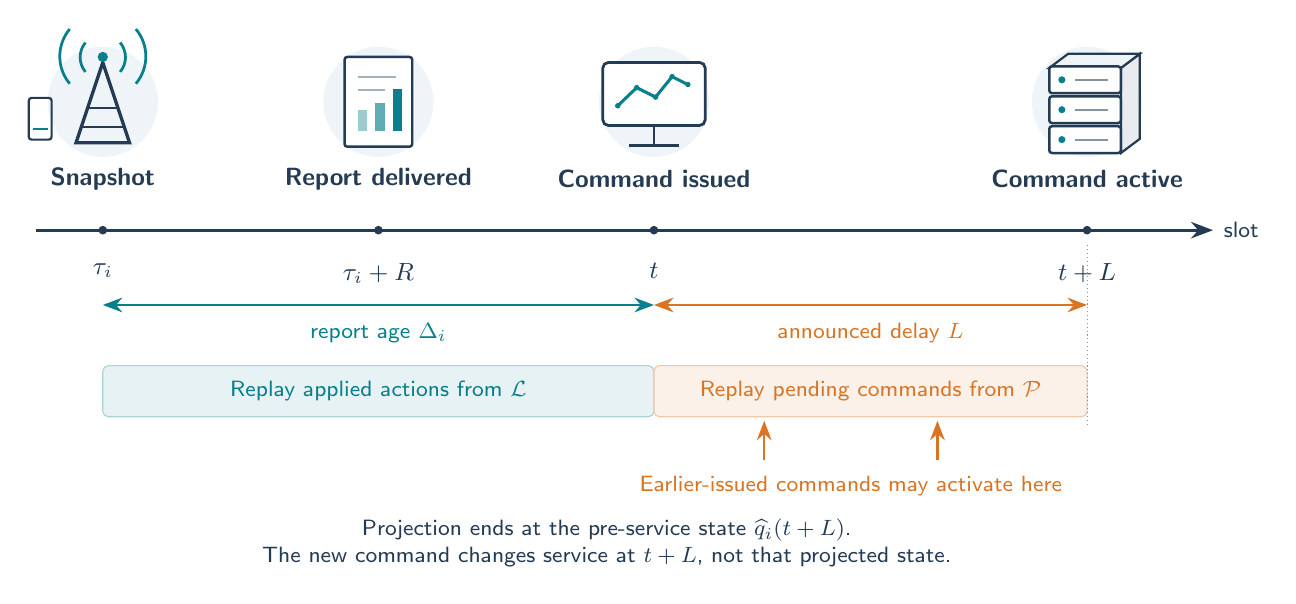
\begin{tikzpicture}[>=Stealth,x=1cm,y=1cm,font=\small\sffamily]
% Four event landmarks use the same icon vocabulary as the architecture.
\foreach \x in {1,4.5,8,13.5}{\path[fill=pale,draw=none] (\x,3.25) circle (.7);}
\pic at (1,3.25) {radio};
\pic at (4.5,3.25) {report};
\pic at (8,3.25) {control};
\pic at (13.5,3.25) {server};
\node[font=\small\sffamily\bfseries,text=ink] at (1,2.27){Snapshot};
\node[font=\small\sffamily\bfseries,text=ink] at (4.5,2.27){Report delivered};
\node[font=\small\sffamily\bfseries,text=ink] at (8,2.27){Command issued};
\node[font=\small\sffamily\bfseries,text=ink] at (13.5,2.27){Command active};
\draw[->,ink,line width=1.1pt] (.15,1.62)--(15.1,1.62) node[right,font=\footnotesize\sffamily]{slot};
\foreach \x/\lab in {1/{$\tau_i$},4.5/{$\tau_i+R$},8/{$t$},13.5/{$t+L$}}{
 \fill[ink] (\x,1.62) circle (.055);
 \node[below=3mm,text=ink] at (\x,1.62){\lab};
}
\draw[<->,signal,line width=.9pt] (1,.67)--node[below=1mm,font=\footnotesize\sffamily]{report age $\Delta_i$}(8,.67);
\draw[<->,command,line width=.9pt] (8,.67)--node[below=1mm,font=\footnotesize\sffamily]{announced delay $L$}(13.5,.67);
\path[fill=signal!10,draw=signal!35,rounded corners=2pt] (1,-.75) rectangle (8,-.10);
\path[fill=command!10,draw=command!40,rounded corners=2pt] (8,-.75) rectangle (13.5,-.10);
\node[text=signal,font=\footnotesize\sffamily] at (4.5,-.42){Replay applied actions from $\mathcal L$};
\node[text=command,font=\footnotesize\sffamily] at (10.75,-.42){Replay pending commands from $\mathcal P$};
\foreach \x in {9.4,11.6}{\draw[->,command,line width=.9pt] (\x,-1.3)--(\x,-.8);}
\node[text=command,font=\footnotesize\sffamily] at (10.5,-1.63){Earlier-issued commands may activate here};
\draw[densely dotted,ink!55] (13.5,-.85)--(13.5,1.45);
\node[align=center,font=\footnotesize\sffamily,text=ink] at (7.4,-2.35)
 {Projection ends at the pre-service state $\widehat q_i(t+L)$.\\The new command changes service at $t+L$, not that projected state.};
\end{tikzpicture}
\caption{Observation-to-activation sequence with explicit equipment roles and action replay. Event positions are schematic. Only already issued commands enter the projection before the new command becomes active.}
\label{fig:timeline}\end{figure*}



Index issued commands by $k$, with issue slot $t_k$, announced delay $L_k$,
activation slot $d_k=t_k+L_k$, expansion $x_k$ and stage-weight matrix $W_k$.
In the proposed controller, each row of $W_k$ is
$(\alpha_k,1-\alpha_k)$. Let command $k=0$ denote the initialized action,
with an activation time before the run. The action active after all due
commands in slot $t$ is characterized by
\begin{equation}
\begin{aligned}
 k^*(t)&=\underset{k:d_k\le t}{\arg\max}_{\rm lex}(d_k,k),\\
 e(t)&=x_{k^*(t)},\qquad W(t)=W_{k^*(t)}.
\end{aligned}
\label{eq:activecommand}
\end{equation}
The lexicographic maximum first selects the latest activation time and then
the latest issue index among simultaneous activations. It is not the latest
issue index across all commands. Consequently, an older command with a larger
delay can overwrite a newer command that became active earlier.

For the ordered list of commands activating in slot $t$, write
$\mathcal K_t=(k_{t,1},\ldots,k_{t,n_t})$, ordered by issue index. Define
$e^{t,0}=e(t-1)$ and $e^{t,j}=x_{k_{t,j}}$ for $j\ge1$, using the initialized
expansion for $e(-1)$. The exact per-slot and full-run costs are
\begin{align}
 j_t&=\sum_i e_i(t)+\kappa\sum_{j=1}^{n_t}
       \|e^{t,j}-e^{t,j-1}\|_1,\label{eq:slotcost}\\
 J&=\sum_{t=0}^{T-1}j_t.\label{eq:commandsumcost}
\end{align}
An empty activation list contributes zero switching cost. The triangle
inequality gives
\begin{equation}
 \sum_{j=1}^{n_t}\|e^{t,j}-e^{t,j-1}\|_1
 \ge\|e(t)-e(t-1)\|_1.
 \label{eq:switchlower}
\end{equation}
Thus charging only the net slot change is a lower bound on the implemented
switching charge. For example, simultaneous changes
$(0,0,0)\rightarrow(0,3,0)\rightarrow(0,0,0)$ incur six switching units,
or cost $1.5$ at $\kappa=0.25$, although the net change is zero.
This distinction matters in J, where multiple commands can activate together.
Equations~\eqref{eq:activecommand}--\eqref{eq:switchlower} explain why a
penalty relative to the previous requested action cannot equal realized
switching cost in every execution.
\subsection{Objective and information-constrained formulation}
The incremental resource objective is
\begin{equation}
 J=\sum_{t=0}^{T-1}\sum_i e_i(t)
 +\kappa\sum_{a\in\mathcal A_T}\norm{x_a-e_a^-},\qquad\kappa=0.25.\label{eq:cost}
\end{equation}
The norm $\lVert z\rVert_1=\sum_i|z_i|$ sums componentwise expansion changes for a vector $z$. The set $\mathcal A_T$ contains all command activations within the run, $x_a$
is the activated expansion, and $e_a^-$ is expansion immediately before that
activation. Every activation is charged, even when several occur in one slot.
The objective includes warm-up and tail capacity, charges actual changes, and
excludes base-resource costs. Initial provisioning incurs no switching charge.
Units are abstract resource cost units, not money, energy or measured power.

For the measured birth cohort $\mathcal C_s$, let $N_s=|\mathcal C_s|$ and let
$\ell_p$ be completion latency. The miss fraction is
\begin{equation}
V_s=\frac{N_s^{\rm late}+N_s^{\rm unfinished}}{\max(1,N_s)}.
\label{eq:miss}
\end{equation}
Here $N_s^{\rm late}$ counts completed cohort packets with $\ell_p>D_s$, and $N_s^{\rm unfinished}$ counts cohort packets unfinished at run end. The tail extends beyond all measured deadlines, so unfinished cohort packets
are known misses rather than right-censored successes. Background arrivals
continue during that tail. Calibration uses a common 0.1\% seed-mean miss screening target for each
class. This finite-sample selection rule is not a chance constraint.





Let $\mathcal I_t$ contain only delivered reports, previously issued commands,
the applied ledger, and the current announced activation delay. A causal policy
$\pi$ maps this information to a command. Let $\Pi$ be the class of such policies
respecting the finite capacity and share grids. For a specified workload law,
the design objective can be written as
\begin{equation}
 \inf_{\pi\in\Pi}\mathbb E_\pi[J]
 \quad\text{subject to}\quad\mathbb E_\pi[V_s]\le\epsilon,
 \qquad s\in\{0,1\}.\label{eq:ideal}
\end{equation}
The expectation is over independent complete runs under that law, matching
the seed-level estimand rather than treating packets as independent trials.
Unobserved packet ages, stochastic ingress and delayed immutable commands
make this a partially observed sequential problem. The proposed controller
does not solve \eqref{eq:ideal}. Instead, Algorithm 1 estimates a future queue,
the finite-grid ranking selects a command from that estimate, and Algorithm 2
screens a fixed policy parameter on separate calibration runs. The test screen
then evaluates its measured cost and miss fractions under each declared law.

This separation has two consequences. First, minimizing the one-step proxy
cost is not minimizing the full-run objective in \eqref{eq:cost}. A switching
penalty relative to the last requested expansion can differ from the actual
activation charge when commands reorder. Second, $\rho_s\le1$ is only a
decision surrogate. It cannot replace the constraint on $V_s$ in
\eqref{eq:ideal}. The model, algorithms and experiments consequently address
three different objects: a design target, an executable approximation, and
finite-sample evidence about that approximation.


To make this information restriction explicit, the packet and command
descriptions can be combined into a state
\begin{equation}
 Z_t=\bigl(X_t,e_t,W_t,\mathcal P_t,\mathcal R_t,\mathcal D_t,
           \mathcal H_t^{\rm meas},\zeta_t\bigr).
 \label{eq:augmentedstate}
\end{equation}
Here $X_t$ collects all age bins, $\mathcal P_t$ stores issued commands awaiting
activation, $\mathcal R_t$ stores reports awaiting delivery, and
$\mathcal D_t$ stores the latest accepted report from each stage.
$\mathcal H_t^{\rm meas}$ contains the finite measurement histories, and
$\zeta_t$ contains the exogenous traffic/capacity state and periodic phase
needed for the selected workload law. State-dependent report construction and
the event order define a transition map
\begin{equation}
 Z_{t+1}=\mathcal F_t(Z_t,u_t,\xi_{t+1}),\qquad
 u_t=\pi_t(\mathcal I_t),\quad\pi\in\Pi_{\mathcal I}.
 \label{eq:causaltransition}
\end{equation}
The random input $\xi_{t+1}$ accounts for exogenous evolution, report loss and
any future announced delays. The action $u_t$ specifies the requested command
and the stage selected for telemetry, and is null outside control epochs.
The information $\mathcal I_t$ consists of delivered reports and their
timestamps, the applied ledger, previously issued commands and the current
announced delay. The set $\Pi_{\mathcal I}$ contains policies measurable with
respect to this information. It excludes access to the hidden age bins and
undelivered reports, even though the simulator retains them for execution.

The objective in \eqref{eq:ideal}, together with
\eqref{eq:agebirth}--\eqref{eq:agemiss} and
\eqref{eq:activecommand}--\eqref{eq:causaltransition}, is therefore a
partially observed, integer-valued sequential resource-allocation problem.
The actual controller compresses $\mathcal I_t$ into projected queue lengths
and a finite-grid score. That compression retains known action effects but
discards the full age distribution and uncertain future arrivals. The expanded
formulation characterizes the underlying problem. The executed algorithm
continues to solve its stated per-decision surrogate, without an additional
stochastic optimizer or an unreported computational benchmark.

\section{Calibrated Action-Aware Controller}
The controller approximates the information-constrained problem using three
steps: reconstruct known action effects, rank a finite set of resource choices,
and select headroom on separate calibration runs. The projection uses only
available information, while the age-resolved model remains the reference for
measuring actual deadline outcomes.

\subsection{Projection from the action ledger}
At decision time $t$, the ledger $\mathcal L(u)$ records the expansion and weights
actually applied at slots $u\le t$. The list $\mathcal P(t)$ contains commands
already issued but not yet activated. Their deterministic activation times
define a known action trajectory up to $t+L-1$. This uses no future exogenous
arrivals or capacity realizations.

For each stage, initialize $\widehat q_i(\tau_i)=q_i$ and hold its latest
reported base capacity and mean ingress constant. The fluid recurrence is
\begin{equation}
\begin{aligned}
 \widehat q_{is}(u+1)&=\left[\widehat q_{is}(u)\right.\\[-2pt]
 &\quad\left.-F_s\bigl(\widehat q_i(u),w_i(u),\bar c_i+e_i(u)\bigr)\right]^+
 +\bar a_{is},\\
 &\qquad u=\tau_i,\ldots,t+L-1.
\end{aligned}
\label{eq:project}
\end{equation}
The fluid service operator $F$ first applies integer reservations, limited by
the real-valued projected workload, and assigns spare units in descending order
of normalized residual workload $(\widehat q_{is}-u_{is})/D_s$. Ties use the class
index. The projection does not contain packet ages, so this borrowing rule is
only an approximation to the packet scheduler.

Each stage is projected independently using its last reported ingress.
Projected upstream departures are not fed into the downstream forecast.
This avoids pretending that asynchronously observed queues constitute a
consistent instantaneous network state, but it also omits propagation of
future upstream actions. The ledger is action-aware, not a perfect network
predictor. The state at $t+L$ is pre-service and therefore excludes the effect
of the new candidate command on that slot's service. Algorithm 1 takes delivered
reports and the action ledger as inputs and returns these activation-time
queue estimates.

\begin{figure}[htbp]\centering
\begin{minipage}{.96\linewidth}
\hrule\smallskip % journal top rule
\textbf{Algorithm 1. Applied-action and pending-command projection}\par\smallskip\hrule\smallskip
\noindent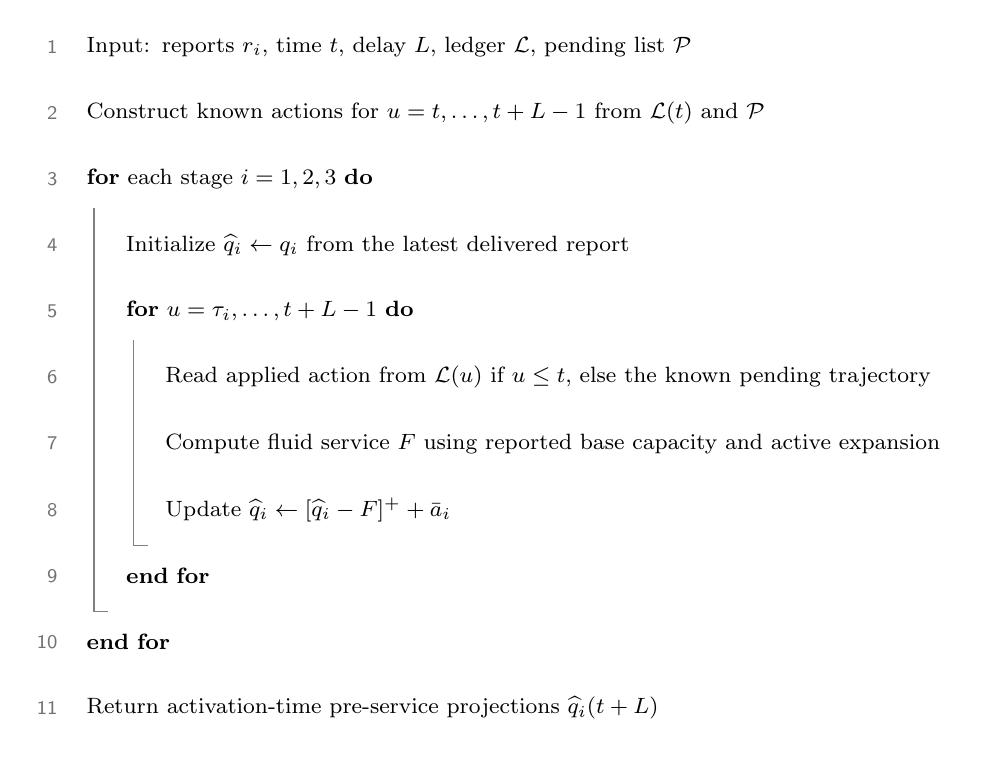
\begin{tikzpicture}[x=1cm,y=1.75cm]
\algline{1}{0}{Input: reports $r_i$, time $t$, delay $L$, ledger $\mathcal L$, pending list $\mathcal P$};
\algline{2}{0}{Construct known actions for $u=t,\ldots,t+L-1$ from $\mathcal L(t)$ and $\mathcal P$};
\algline{3}{0}{\textbf{for} each stage $i=1,2,3$ \textbf{do}};
\algline{4}{.5}{Initialize $\widehat q_i\leftarrow q_i$ from the latest delivered report};
\algline{5}{.5}{\textbf{for} $u=\tau_i,\ldots,t+L-1$ \textbf{do}};
\algline{6}{1}{Read applied action from $\mathcal L(u)$ if $u\le t$, else the known pending trajectory};
\algline{7}{1}{Compute fluid service $F$ using reported base capacity and active expansion};
\algline{8}{1}{Update $\widehat q_i\leftarrow [\widehat q_i-F]^++\bar a_i$};
\algline{9}{.5}{\textbf{end for}};
\algline{10}{0}{\textbf{end for}};
\algline{11}{0}{Return activation-time pre-service projections $\widehat q_i(t+L)$};
\draw[gray] (.17,-1.65)--(.17,-4.58)--(.35,-4.58);
\draw[gray] (.67,-2.61)--(.67,-4.1)--(.85,-4.1);
\end{tikzpicture}\hrule
\end{minipage}
\end{figure}

\subsection{Finite-grid allocation and sensitivity}
The bounded-horizon demand proxy is
\begin{equation}
 d_{is}=\widehat q_{is}(t+L)+h\bar a_{is}+\sqrt{h v_{is}}+1.\label{eq:demand}
\end{equation}
The square-root term is a dispersion heuristic evaluated over one control
interval. It is not a confidence bound on the longer queue-projection horizon.
The additive one-packet term is a fixed conservative offset. Both are explicit
design choices, not parameters inferred from O-RAN measurements.

The decision grid contains
\begin{equation}
 \begin{gathered}\mathcal X=\{((0,x_2,x_3),k/20):\\ x_2,x_3\in\{0,1,2,3\},\ k\in\{1,\ldots,19\}\},\\|\mathcal X|=304.\end{gathered}
\end{equation}
The same share is applied at all stages. With reported base capacities,
candidate integer reservations and headroom $\eta$ yield
\begin{align}
 \rho_s(x,\alpha)&=\frac1{\eta D_s}\sum_i
 \frac{d_{is}}{\max\{10^{-3},g_{is}(\bar c_i+x_i,\alpha)\}},\\
 r(x,\alpha)&=\max_s\rho_s(x,\alpha),\\
 c(x)&=\sum_i x_i+\kappa\norm{x-x^{\mathrm{req}}_{\mathrm{prev}}}.\label{eq:proxycost}
\end{align}
The small denominator floor defines a finite penalty for zero reservations,
not guaranteed fractional service. The cost proxy compares with the previous
\emph{requested} expansion. It differs intentionally from the realized cost in
\eqref{eq:cost}, which uses actual activation changes.

Candidates are ranked lexicographically by
\begin{equation}
 \sigma(x,\alpha)=
 \begin{cases}
 (0,c,r,\sum_s\rho_s,k), & r\le1,\\
 (1,r,c,\sum_s\rho_s,k), & r>1.
 \end{cases}\label{eq:ranking}
\end{equation}
The minimum is selected, retaining the earliest enumerated expansion on any
remaining tie. Feasible candidates prioritize cost. When none is feasible,
the least worst-class ratio is selected. No claim of feasibility is made for
the realized packet system from this surrogate decision.




The ranking can be interpreted through its workload-to-service ratio.
For a fixed report state, define the unscaled service-time proxy
\begin{equation}
 H_s(x,\alpha)=\sum_{i=1}^{3}\frac{d_{is}}{\widetilde g_{is}},
 \qquad \widetilde g_{is}=\max\{10^{-3},g_{is}(\bar c_i+x_i,\alpha)\}.
 \label{eq:worktime}
\end{equation}
The quantity $\widetilde g_{is}$ is the floored reservation denominator used
in the implemented ranking. Dividing packet workload $d_{is}$ by reserved
packets per slot gives a stage service-time proxy. Adding the stage proxies
gives $H_s$ in slots. This algebra does not incorporate the packet ages or
joint stage dynamics required for a true end-to-end delay bound. The controller
normalizes this proxy by the headroom-adjusted deadline:
\begin{equation}
\begin{gathered}
 \rho_s=H_s/(\eta D_s),\\
 \mathcal F(\eta)=\{(x,\alpha)\in\mathcal X:\rho_s\le1\ \forall s\}.
\end{gathered}
\label{eq:feasibleset}
\end{equation}
For the same reports and candidate actions, $0<\eta_1\le\eta_2$ implies
$\mathcal F(\eta_1)\subseteq\mathcal F(\eta_2)$. Thus reducing $\eta$ cannot
create a newly feasible candidate at that decision state. If both sets are
nonempty, the minimum feasible proxy cost cannot decrease when $\eta$ is
reduced. This local statement does not imply monotone realized cost over a
closed-loop run, where actions also change future reports and queues.

Holding the projected state and reservations fixed, the corresponding local
sensitivities are
\begin{align}
 \frac{\partial\rho_s}{\partial\eta}&=-\frac{\rho_s}{\eta},&
 \frac{\partial\rho_s}{\partial\widehat q_{is}}&=\frac{1}{\eta D_s\widetilde g_{is}},
 \label{eq:etasensitivity}\\
 \frac{\partial\rho_s}{\partial v_{is}}&=
 \frac{\sqrt h}{2\eta D_s\widetilde g_{is}\sqrt{v_{is}}},\qquad v_{is}>0.
 \label{eq:variancesensitivity}
\end{align}
These derivatives describe the score between changes in integer reservations.
They are not derivatives of the selected action, which can jump between grid
points. Equation~\eqref{eq:etasensitivity} explains why headroom can exclude
cheap candidates, while \eqref{eq:variancesensitivity} identifies the greater
sensitivity associated with small reservations and short deadlines. At zero
variance the square-root term is continuous but its derivative is not finite.


The ranking is discrete, so a smooth derivative alone cannot describe its
response to one added capacity unit. For two classes with integer total
capacity $C$ and weights $(w_0,w_1)=(\alpha,1-\alpha)$, define proportional
quotas $r_s=Cw_s/(w_0+w_1)$, fractional parts $f_s=r_s-\lfloor r_s\rfloor$
and remainder $\nu=C-\sum_s\lfloor r_s\rfloor$. Largest-remainder allocation gives
\begin{equation}
\begin{aligned}
 g_0(C,\alpha)&=\lfloor r_0\rfloor+\nu\mathbf1\{f_0\ge f_1\},\\
 g_1(C,\alpha)&=C-g_0(C,\alpha).
\end{aligned}
\label{eq:integerquota}
\end{equation}
To obtain this expression, floor both proportional quotas and allocate any
remaining unit to the larger fractional part, using class index for equality.
This explains the plateaus and jumps as $\alpha$ changes. In exact arithmetic,
$g_0=\lfloor\alpha C+1/2\rfloor$. Reproduction uses the computed fractional
parts instead: binary floating-point values can distinguish a mathematical
tie. For example, the saved implementation returns $(3,2)$ at $C=5$ and
$\alpha=0.70$. The executed allocation routine is retained unchanged, and
\eqref{eq:integerquota} is checked against it throughout the relevant grid.

For fixed demand and a fixed share, compare candidate capacities $C_i$ and
$C_i+1$. Define the corresponding floored denominators as
$\widetilde g_{is}$ and $\widetilde g'_{is}$, as in
\eqref{eq:worktime}. Their exact contribution to the class-score change is
\begin{equation}
 \rho_s'-\rho_s
 =-\frac{d_{is}(\widetilde g'_{is}-\widetilde g_{is})}
 {\eta D_s\widetilde g_{is}\widetilde g'_{is}}.
 \label{eq:discretemarginal}
\end{equation}
This follows by subtracting the two reciprocal service terms. An added unit
can leave one class's score unchanged if its reservation does not increase.
Its effect is amplified when it removes a zero reservation, where the numerical
denominator floor is active. Thus a common share and an integer service budget
couple the two classes even though the score is computed classwise. The
quantity in \eqref{eq:discretemarginal} is a proxy improvement, not an observed
change in packet latency.

The score also permits a finite perturbation bound. At fixed candidate
reservations, let $E^q_{is}$, $E^a_{is}$ and $E^v_{is}$ bound the absolute
differences between two projected queues, mean-ingress estimates and
nonnegative net-flow variance estimates. From \eqref{eq:demand}, the triangle
inequality and $|\sqrt{v'}-\sqrt v|\le\sqrt{|v'-v|}$ give
\begin{align}
 |d'_{is}-d_{is}|&\le E^q_{is}+hE^a_{is}+\sqrt{hE^v_{is}},
 \label{eq:demanderror}\\
 |\rho_s'-\rho_s|&\le B_s
 :=\frac1{\eta D_s}\sum_i
 \frac{E^q_{is}+hE^a_{is}+\sqrt{hE^v_{is}}}{\widetilde g_{is}}.
 \label{eq:scoreerror}
\end{align}
If such bounds were available and $\rho_s+B_s\le1$ for both classes, the
same candidate would remain surrogate-feasible under those perturbations.
No such error bounds were calibrated or enforced in the executed controller.
This is an analytical diagnostic, not a newly implemented robust policy.

Equation~\eqref{eq:scoreerror} connects the sensitivity analysis to the test
design. At equal reservations and error magnitudes, the shorter deadline
$D_0=15$ amplifies score perturbations by $D_1/D_0=8/3$ relative to $D_1=40$.
Meanwhile, the projection horizon is $\Delta_i+L$, but the dispersion allowance
uses only $h=5$. Increasing $L$ therefore extends exposure to unmodeled
ingress changes without automatically enlarging that allowance. The ledger
removes ambiguity about known actions, not uncertainty about future traffic.
This distinction motivates examining both proxy-feasibility frequency and
actual misses in the results.
\subsection{Calibration, execution and comparison policies}
Let $\eta\in\{0.25,0.5,0.75,1\}$ be a dimensionless headroom parameter.
The ratios in the ranking are divided by $\eta$, so smaller values impose a
stricter surrogate-feasibility threshold. They do not impose a hard constraint
on realized packet misses. The control interval, dispersion term and candidate
grid remain fixed across the headroom candidates.

For each policy family $m$ and candidate parameter $\theta$, calibration
estimates the seed mean of each class miss fraction in two report-quality
strata. Let $U_{m\theta cs}$ be its one-sided 95\% percentile-bootstrap upper
endpoint, where $c$ identifies the stratum and $s$ the class. Selection is
\begin{equation}
\begin{aligned}
 \theta_m^*&=\arg\min_{\theta\in\Theta_m}\overline J_{m\theta}\\
 &\text{subject to }U_{m\theta cs}\le\epsilon\quad\forall c,s,\\
 &\epsilon=10^{-3}.
\end{aligned}
\label{eq:calibration}
\end{equation}
The finite set $\Theta_m$ contains the candidate parameters for family $m$. Here $\overline J$ averages calibration costs across both strata. The threshold
is a 0.1\% seed-mean miss target, not a per-packet chance guarantee or an
O-RAN service-level specification. If a family has no passing candidate, it
is explicitly marked calibration-ineligible and its prespecified conservative
endpoint is retained for diagnosis only. No hidden fallback is substituted
into the proposed policy during a test run.


The same calibration rule is applied to the following comparison families.
The fixed family enumerates all sixteen profiles $(0,x_2,x_3)$ on the same
calibration seeds. It starts preprovisioned and retains the earlier drift-based
share controller. It does not use future traffic, but its known bottleneck
location is used to transpose the selected profile for the compute case.
Consequently, the fixed comparison evaluates complete policies, not the
isolated effect of capacity switching under identical class shares.

The HPA-inspired adaptation computes a target expansion at each expandable
stage using target utilization $u$:
\begin{equation}
\begin{aligned}
 b_i(t)&=\left[\left\lceil\frac{\sum_s\bar a_{is}+\sum_s q_{is}/h}{u}\right\rceil-\bar c_i\right]_0^3,\\
 x_i(t)&=\max_{v\in\mathcal H_t}b_i(v).
\end{aligned}
\label{eq:hpa}
\end{equation}
The clipping operator $[z]_0^3$ limits $z$ to $[0,3]$, and $\mathcal H_t$
contains recommendations generated in the last twenty slots. Stage 1 has
zero expansion. Candidate utilizations are $0.55,0.70,0.85,0.95$. Queue
clearance over $h$ slots is a task-specific addition to ratio-based sizing.
The common finite-grid share ranking with $\eta=1$ selects weights for this
fixed target capacity, using the drift projection rather than the action
ledger. This is neither a Kubernetes deployment nor its default timing.

The DPP-inspired adaptation uses a price $v\in\{0.1,0.3,1,3\}$ and selects
the candidate minimizing
\begin{equation}
 v c(x)-\sum_{i,s}\frac{\widetilde q^{L}_{is}+h\bar a_{is}}{D_s}
       \min\{d^{\mathrm{drift}}_{is},g_{is}(\bar c_i+x_i,\alpha)\}.
 \label{eq:dpp}
\end{equation}
Here $\widetilde q^{L}_{is}=[q_{is}+(\Delta_i+L)(\bar a_{is}-\bar\mu_{is})]^+$,
and $d^{\mathrm{drift}}$ replaces the action-aware queue in
\eqref{eq:demand} with that drift projection. Cost breaks objective ties,
followed by share index and enumeration order. Deadline normalization and
clipped service rewards are explicit adaptations. No virtual deadline-deficit
queues, backpressure differentials or imported Lyapunov guarantee are claimed.
A failed calibration for this adaptation is not evidence against the broader
DPP method family.

Two internal ablations complete the comparison. \emph{Uncalibrated} uses the
action ledger with $\eta=1$. \emph{No ledger} uses the selected headroom but
substitutes $\widetilde q^{L}$ for the action-aware projection. The latter
isolates projection effects at a common headroom parameter, not an independently
optimized alternative policy family. Algorithm 2 separates the offline
selection of parameters from online command execution. The selected parameters
remain locked throughout the held-out evaluation.

\begin{figure}[htbp]\centering
\begin{minipage}{.96\linewidth}
\hrule\smallskip % journal top rule
\textbf{Algorithm 2. Reliability-screened selection and elastic execution}\par\smallskip\hrule\smallskip
\noindent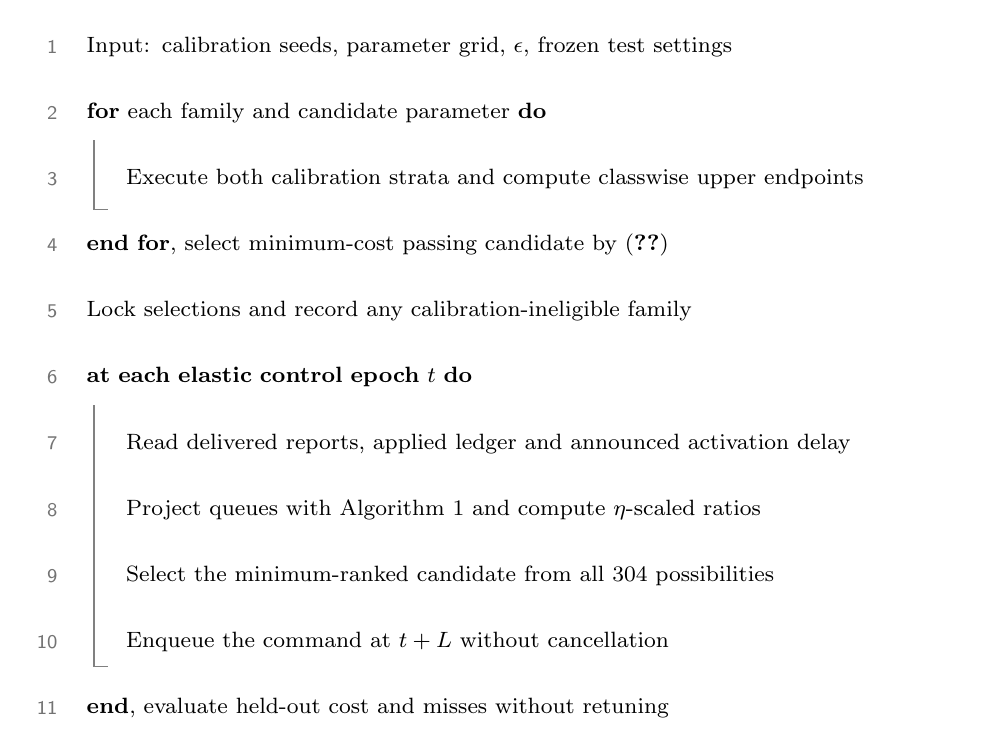
\begin{tikzpicture}[x=1cm,y=1.75cm]
\algline{1}{0}{Input: calibration seeds, parameter grid, $\epsilon$, frozen test settings};
\algline{2}{0}{\textbf{for} each family and candidate parameter \textbf{do}};
\algline{3}{.5}{Execute both calibration strata and compute classwise upper endpoints};
\algline{4}{0}{\textbf{end for}, select minimum-cost passing candidate by (\ref{eq:calibration})};
\algline{5}{0}{Lock selections and record any calibration-ineligible family};
\algline{6}{0}{\textbf{at each elastic control epoch} $t$ \textbf{do}};
\algline{7}{.5}{Read delivered reports, applied ledger and announced activation delay};
\algline{8}{.5}{Project queues with Algorithm 1 and compute $\eta$-scaled ratios};
\algline{9}{.5}{Select the minimum-ranked candidate from all $304$ possibilities};
\algline{10}{.5}{Enqueue the command at $t+L$ without cancellation};
\algline{11}{0}{\textbf{end}, evaluate held-out cost and misses without retuning};
\draw[gray] (.17,-1.16)--(.17,-1.66)--(.35,-1.66);
\draw[gray] (.17,-3.08)--(.17,-4.98)--(.35,-4.98);
\end{tikzpicture}\hrule
\end{minipage}
\end{figure}

\section{Formal Properties and Limits}
The preceding construction supports exact statements about information use,
packet conservation and the finite-grid decision. These properties are followed
by deadline-capacity bounds that identify what even a better ranking rule cannot
repair once the remaining service opportunities are insufficient.

\begin{proposition}[Causality]
For fixed configuration and initialization, every elastic decision at time $t$
is a function only of reports delivered by $t$, commands already issued and
their known activation times. It is independent of unobserved future traffic
and base-capacity realizations.
\end{proposition}
\begin{proof}
The report selector reads only stored payloads and their timestamps. The ledger
contains previously applied commands. The pending list contains commands issued
at earlier epochs. Equation~\eqref{eq:project} uses these actions and holds
reported base capacity and ingress fixed. The demand and ranking equations are
deterministic functions of that projection. Induction over decision epochs
therefore excludes future exogenous trace entries. A future-suffix perturbation
test additionally checks this property in the executable implementation.
\end{proof}

\begin{proposition}[Conservation and service bounds]
For every slot, all queues remain nonnegative, stage service does not exceed
available capacity, and the total number of generated packets equals completed
packets plus packets remaining in the chain. Completed latency is at least
three slots.
\end{proposition}
\begin{proof}
Reservations are limited by available queue contents. Borrowing only selects a
class with a remaining packet and stops at capacity, proving nonnegativity and
the service bound. Summing \eqref{eq:q1}--\eqref{eq:qi} cancels each internal
transfer, leaving external arrivals minus final-stage completions. Induction
from empty queues proves conservation. Reverse stage order prevents a packet
from receiving two stages of service in one slot, giving the latency bound.
\end{proof}

\begin{proposition}[Finite-grid decision optimality]
The enumerator returns a minimum of \eqref{eq:ranking} on $\mathcal X$.
If any surrogate-feasible candidate exists, the result is surrogate-feasible
and has minimum proxy cost among all such candidates.
\end{proposition}
\begin{proof}
All sixteen expansion vectors and nineteen share values are visited. The
running incumbent changes only for a strictly smaller lexicographic score.
After the last candidate it is a minimum over the complete finite set. The
leading score component ranks every feasible candidate ahead of every infeasible
candidate, and cost is the first varying component within the feasible subset.
This establishes the stated result, not global stochastic-control optimality.
\end{proof}


\begin{proposition}[Actuation irreversibility]
Consider two executions with identical exogenous traces, initial states and
all applied actions before slot $a$. A command that first changes an action
at slot $a$ cannot change the on-time-completion indicator of any packet whose
absolute deadline is strictly earlier than $a$.
\end{proposition}
\begin{proof}
The deterministic event contract gives identical packet states and service
decisions through slot $a-1$ by induction. Every completion opportunity up to
the stated packet deadline is therefore identical. A change beginning at
$a$ cannot alter whether the packet completed by an earlier slot.
\end{proof}
In particular, a decision issued at $t$ with activation $t+L$ cannot rescue a
packet with deadline below $t+L$ unless other already-scheduled actions do so.
This structural observation is not a novel stability theorem. It explains why
more accurate accounting of pending actions cannot remove arbitrarily long
actuation latency. Preprovisioning, predictive information before the burst,
or a faster local mechanism is required to change those earlier opportunities.


\subsection{Deadline limits and computational cost}
Age resolution sharpens the aggregate capacity obstruction. At a pre-service
slot $t$, consider measured-cohort packets currently waiting at stages
$j\le i$ whose absolute deadlines are no later than $d$, with $t\le d<T$.
Their count is
\begin{equation}
 B_i^{\mathcal C}(t,d)=
 \sum_{j=1}^{i}\sum_{s,a}
 \chi(t,a)\mathbf1\{t-a+D_s-1\le d\}X_{jsa}(t).
 \label{eq:deadlinedemand}
\end{equation}
Every such packet still needs stage-$i$ service. Because the remaining
$3-i$ stages each require a later slot, it must leave stage $i$ no later
than $d-(3-i)$. Even if all available service were assigned to these packets,
their on-time completion count cannot exceed
\begin{equation}
 K_i(t,d)=\sum_{u=t}^{d-(3-i)}C_i(u),
 \label{eq:deadlinecapacity}
\end{equation}
with an empty sum interpreted as zero. Let $M^{\mathcal C}(t,d)$ denote the
eventual number of misses among currently queued cohort packets with deadline
at most $d$. The necessary pathwise inequality is
\begin{equation}
 M^{\mathcal C}(t,d)\ge
 \max_{i\in\{1,2,3\}}[B_i^{\mathcal C}(t,d)-K_i(t,d)]^+.
 \label{eq:misscut}
\end{equation}
To prove the inequality, each on-time packet in the stage-$i$ subset must
consume one distinct service unit in its stated window. At most $K_i$ such
units exist, leaving at least $[B_i^{\mathcal C}-K_i]^+$ misses. The maximum
combines valid lower bounds without counting the same packet multiple times.
The bound relaxes upstream release times, other traffic and reserved shares,
so a zero value does not establish feasibility. Unlike a steady-state load
condition, it retains residual deadlines and downstream transit time.

For the constant-delay cases, no command issued at or after $t$ changes
capacity before $t+L$. Let $e_i^{\rm pend}(u)$ be the expansion obtained by
replaying the applied action and commands already issued before $t$, and let
$e_i^{\max}$ be $0$ for stage 1 and $3$ otherwise. A control-independent upper
envelope on capacity opportunities is
\begin{equation}
 \overline K_i(t,d)=\sum_{u=t}^{d-(3-i)}
 \left[c_i(u)+
 \begin{cases}
 e_i^{\rm pend}(u),&u<t+L,\\
 e_i^{\max},&u\ge t+L.
 \end{cases}\right].
 \label{eq:delaycut}
\end{equation}
Since $K_i\le\overline K_i$, substituting $\overline K_i$ into
\eqref{eq:misscut} gives a lower bound valid for every subsequent admissible
control sequence under that fixed-delay assumption. Future base capacities
are not observed by the controller, so this is a pathwise analytical bound,
not an implemented online certificate. In J, later-issued commands can have
shorter delays. The fixed-$L$ envelope must not be applied to that case.

A necessary condition for all packets in any cohort to meet their deadlines
is that each stage has enough cumulative service opportunities within the
union of their allowable residence intervals. In particular, if a cohort born
in $[a,b]$ has $N$ packets and maximum deadline $D_{\max}$, then
\begin{equation}
 N\le\sum_{t=a}^{b+D_{\max}-1} C_i(t)\qquad\text{for every stage }i.\label{eq:cut}
\end{equation}
Every such packet must consume one unit at every stage within that interval.
Violation of \eqref{eq:cut} therefore precludes universal deadline satisfaction.
The condition is loose and not sufficient because it ignores class deadlines,
competing packets, stage precedence and service timing.

For disjoint service windows $I_j=[a_j,b_j+D_{\max}-1]$ containing
cohorts of size $N_j$, the same argument gives the zero-miss necessary cost bound
\begin{equation}
 J\ge\sum_i\sum_j\left[N_j-\sum_{t\in I_j}c_i(t)\right]^+.
\end{equation}
Disjointness prevents counting the same capacity opportunity twice. This lower
bound omits switching charges, competing traffic and precedence, so it is not
an achievable optimum. It applies to zero misses for those cohorts, not to
the relaxed empirical target in this experiment. No approximation ratio or
optimality gap is inferred from it.

With two classes and three stages fixed, projection work scales with
$\sum_i(\Delta_i+L)$. The grid requires 304 candidate scores, with reusable
stage/share calculations. In the general $m$-stage extension with $E+1$
expansion levels at each expandable stage and $K$ shares, exhaustive selection
scales as $O(K(E+1)^{m-1}mS)$ for $S$ classes. Thus the small present grid is
not evidence of scalability to many independent resource domains. The reference
implementation retains a full applied-action ledger. A production implementation
could discard entries older than the oldest stored report, subject to its report
delivery contract. No wall-clock real-time feasibility claim is made.



\section{Experimental Method}
The experiments test the distinction established by the analysis: a causal,
surrogate-optimal decision need not meet packet deadlines. Nominal runs measure
cost under the common reliability screen, shifted workloads probe the deadline
limits, and ablations isolate the roles of headroom and action memory.

\subsection{Workloads and experimental controls}
Each run has 3340 slots: 300 warm-up slots, a 3000-slot measured birth cohort,
and a forty-slot tail. Background traffic continues during the tail. The class
deadlines are $(15,40)$ slots. An illustrative mapping of twenty milliseconds
per slot gives 300 and 800 milliseconds, not ultra-reliable low-latency communication (URLLC) deadlines. No measured
mapping from packet units to physical resource blocks or central processing unit (CPU) cycles is used.

\begin{table*}[htbp]\centering\small
\caption{Fixed parameters and complete held-out matrix. Each setting runs six methods on twenty seeds.}
\begin{tabular}{p{31mm}p{116mm}}\toprule
Item & Specification\\\midrule
Common model & Three stages, two classes, $h=5$, $W=20$, $\kappa=0.25$\\
Base capacity & $5+\xi$ per stage, $\xi$ sampled from $(-1,0,0,1)$\\
Periodic bursts & Means $(0.9,2.1)$ outside and $(1.8,3.8)$ inside $t\bmod600\in[180,290)$\\
Capacity stress & Stage 2 capacity $3$ during $t\bmod600\in[170,310)$\\
Initialization & Queue $(0,0)$, ingress $(0.9,2.1)$, service $(2.5,2.5)$, variance $(1,1)$, capacity $5$\\
P & Periodic bursts, transport stress, $(R,p,L)=(3,0.05,10)$\\
M & Markov-modulated Poisson traffic and transport stress, $(3,0.05,10)$\\
B & Markov-modulated batches of three, same conditional means, $(3,0.05,10)$\\
C & Periodic bursts with stress relocated to stage 3, $(3,0.05,10)$\\
R & Periodic transport stress with degraded reports, $(9,0.15,10)$\\
L & Periodic transport stress, long actuation delay, $(3,0.05,50)$\\
J & Periodic transport stress, $(R,p)=(3,0.05)$, announced $L\in\{1,5,10,25,50\}$\\\bottomrule
\end{tabular}\label{tab:settings}
\end{table*}

For M and B, a two-state chain begins in the low state. At each slot its
low-to-high probability is 0.005 and its high-to-low probability is 0.02.
Poisson arrival means in each state equal the corresponding nominal and burst
means above. Transport capacity is three in the high state and fluctuating
base capacity in the low state. Other stages retain the exogenous base-capacity
draws. In B, the number of arriving batches is Poisson with mean one third of
the conditional packet rate, and each batch contains three packets. Thus B
preserves conditional means but increases conditional variance. These cases
alter both burst timing and its correlation with transport capacity. They
are synthetic distribution shifts, not independent real-network datasets.

In J, every command delay is sampled uniformly from $\{1,5,10,25,50\}$ and
announced when that command is issued. Controllers do not see future delay
draws. All methods share the same delay sequence within a seed. The mean delay
is 18.2 slots, so P versus J is not a pure variance comparison at equal mean.
Multiple commands can activate in one slot, in issuance order. Commands with
longer delays may activate after subsequently issued commands. They are not
silently canceled or superseded.


The local protocol, parameter grids and failure rule were written before these
calibration and test executions. It is not an externally registered protocol.
Calibration seeds 12000--12005 are distinct from test seeds 13000--13019.
The two calibration strata are P and R, each at ten-slot actuation delay.
Sixteen fixed profiles plus four candidates for each of the three elastic
families give $(16+4+4+4)\times2\times6=336$ calibration executions.
After selection, seven settings, six methods and twenty seeds give 840 test
executions. All six methods use the same seed-specific exogenous trace, the
same request-index loss flags and one request every five slots. Trace hashes,
admitted cohort counts and delivered-report counts are checked for equality.
Different methods can select different report stages, so payloads need not
be identical. Fixed provisioning has a larger calibration search budget than
each elastic family. Each family has only one selected test configuration.

The prespecified diagnostic fallback parameters are fixed $(3,3)$, headroom
$0.25$, utilization $0.55$ and DPP price $0.1$. They are used only when the
corresponding family has no passing calibration candidate, and that status
remains visible. The earlier 800-run delay-gated study is retained in the
archive as development history. Its seeds and results are not pooled with
the current experiment, and its 1\% calibration target is not reused.

\subsection{Statistical evaluation and verification}
The independent replication unit is a complete seed, not a packet. Results
average seed-level miss fractions and costs. Two-sided 95\% percentile-bootstrap
intervals use 10,000 seed resamples \cite{efron}. One-sided upper endpoints
use the 95th percentile of 10,000 bootstrap means. Paired comparisons resample
within-seed differences. Packet dependence within a run is therefore not
mistaken for thousands of independent trials.

For a proposed-versus-reference comparison in setting $c$, a qualified cost
advantage requires: both families passed calibration, both test upper
endpoints satisfy $U_{cs}\le\epsilon$ for both classes, the upper endpoint
of each paired miss difference is at most $\delta=10^{-3}$, and the upper
endpoint of the paired cost difference is negative. The margin $\delta$ is
0.1 percentage point. This is descriptive noninferiority screening under
common thresholds, not equality of reliability or a guaranteed safety claim.
Internal ablations are displayed as diagnostic comparisons, not separately
calibrated deployment families.

These intervals are unadjusted across settings, classes, candidates and
comparators. No familywise confirmatory significance claim is made. The sequential multiplicity-adjustment procedure in \cite{holm} was used for the archived study's separate sign-test
family, not retroactively applied to these bootstrap screens. Calibration
selection and the small six-seed calibration sample can overfit the screen.
Fresh test seeds mitigate reuse of outcomes but do not remove finite-sample
uncertainty or protect against distribution shift.

An all-zero sample gives a zero-width percentile interval. It does not prove
zero risk. With zero seeds exhibiting any miss among twenty independent,
identically distributed test seeds, an exact one-sided 95\% binomial upper
bound for the probability that a whole run exhibits any miss is
$1-0.05^{1/20}=0.1391$. This is a \emph{run-event} bound, not a packet-miss
bound. The all-zero bootstrap result is consequently treated as a descriptive
screen, not a rare-event certificate.


Verification links this statistical protocol back to the mathematical
model. Independent age-bin reconstruction checks six complete executions and
306 stage/deadline cuts against frozen outcomes.
The release runs 51 unit-test methods, historical-regression checks, an
independent packet replay and complete reconciliation of all 1176 new
execution records. Tests include uncached finite-grid enumeration, constant
delay regression, variable-delay activation order, future-trace exclusion,
compound-arrival construction and independent replay under jitter.
Six selected full test runs are regenerated and compared exactly to saved
records. Mathematical cost definitions include every applied command change,
including multiple changes within a slot. Tables and vector plots are built
directly from execution records in JavaScript Object Notation (JSON). The final Portable Document Format (PDF) file is compiled to resolved references
and checked separately from its intermediate build passes.


\section{Results and Mechanistic Interpretation}
The results follow the evaluation protocol in three stages. Calibration and
held-out screening first identify admissible cost comparisons. Traffic and delay
shifts then expose failures. Finally, ablations connect those outcomes to the
capacity, switching and workload terms in the model.


The selected fixed expansion is $(x_2,x_3)=(2,0)$, the selected headroom is
$\eta=0.75$, and the selected utilization is $u=0.85$. No DPP-inspired candidate
passes both calibration strata, so price $v=0.1$ remains diagnostic only.
Figure~\ref{fig:calibration} reports all candidates, including failed choices.
The three lower headroom values pass the empirical calibration screen. The
$\eta=1$ variant does not. Selection minimizes cost among passing grid points,
not over an unknown continuous optimum or a confidence-certified feasible set.
\begin{figure*}[htbp]\centering
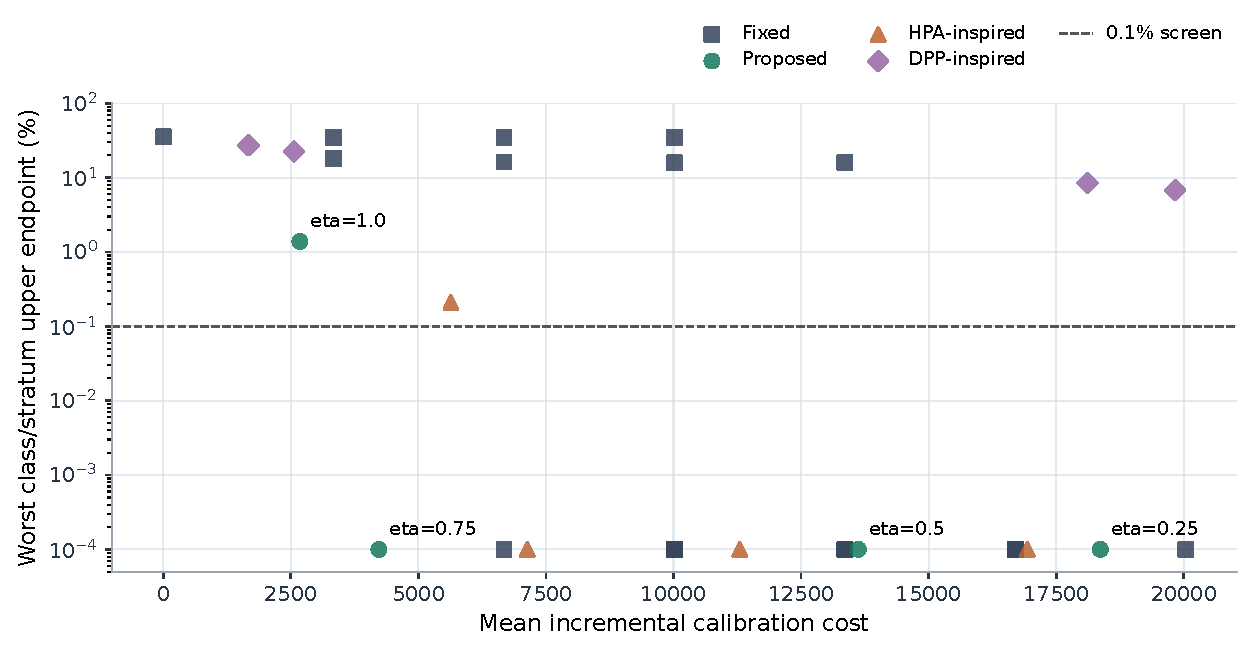
\includegraphics[width=.96\linewidth]{calibration.pdf}
\caption{Calibration cost and worst class/stratum upper endpoint. Each marker
represents one candidate evaluated on twelve runs. The horizontal line is the
0.1\% screening target. Points below the display floor represent zero empirical
endpoints, not certified zero risk.}
\label{fig:calibration}
\end{figure*}
Table~\ref{tab:headroom} and Figure~\ref{fig:headroom} isolate the headroom sweep
on identical calibration seeds. Tightening $\eta$ contracts the candidate set
in \eqref{eq:feasibleset}, which is consistent with higher observed resource
cost. The values $0.25$ and $0.50$ purchase substantially more capacity than
$0.75$ without improving their already-zero empirical miss endpoints. Those
zeros do not establish equal true risk. At $\eta=1$, reduced provisioning is
accompanied by failed endpoints. The trade-off is therefore substantive, not
merely a tunable score with no connection to packet outcomes.
\begin{table*}[htbp]\centering\small
\caption{Headroom sensitivity on calibration seeds. Upper endpoints are percentages.}\label{tab:headroom}
\begin{tabular}{rrrrl}\toprule $\eta$ & Mean cost & Upper $V_0$ & Upper $V_1$ & Eligible\\\midrule
0.25 & 18365.44 & 0.0000 & 0.0000 & Yes \\
0.50 & 13621.71 & 0.0000 & 0.0000 & Yes \\
0.75 & 4226.92 & 0.0000 & 0.0000 & Yes \\
1.00 & 2678.08 & 0.7315 & 1.3879 & No \\
\bottomrule\end{tabular}\end{table*}\begin{figure*}[htbp]\centering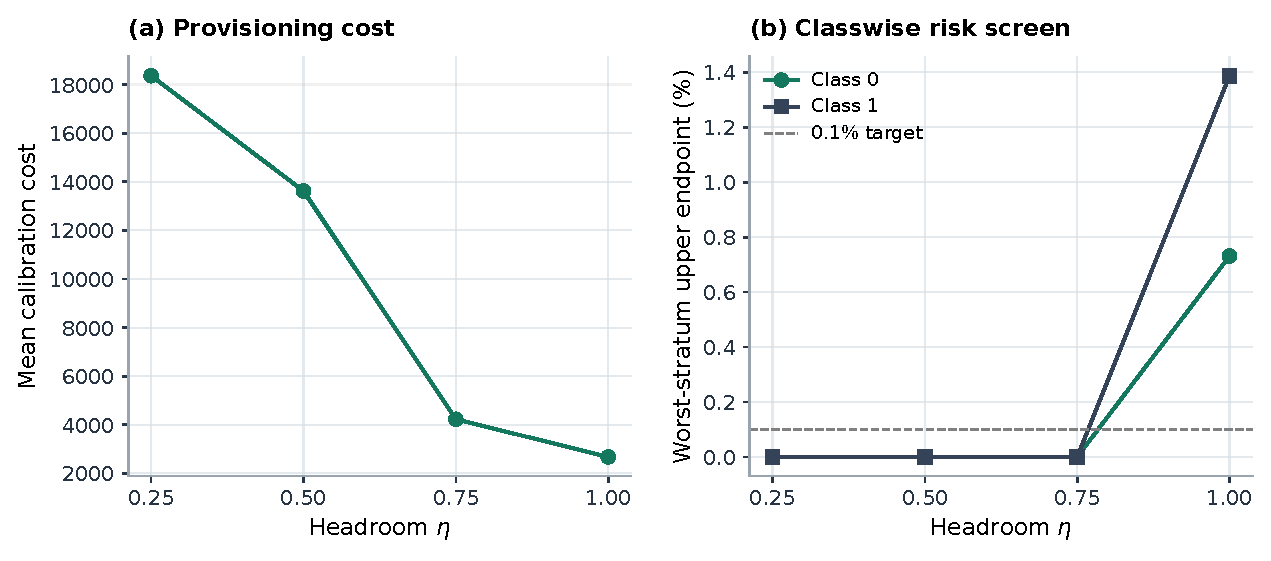
\includegraphics[width=.96\linewidth]{headroom_sensitivity.pdf}
\caption{Sensitivity to headroom on the frozen calibration grid. Left: mean incremental cost. Right: worst-stratum classwise upper endpoints. The dashed line marks the empirical screening target.}\label{fig:headroom}\end{figure*}


Figure~\ref{fig:screen} renders every part of the unchanged comparison rule.
The paired cost condition passes in all seven settings. Reliability, not the
sign of the cost difference, determines which savings can be qualified.
P, R and J pass every condition. M, B and L fail the proposed absolute-risk
screen, while C fails because the fixed reference exceeds its class-1 target.
This is why the zero observed misses of the proposed policy in C do not
produce a qualified comparison under the declared rule.
\begin{figure*}[!htbp]\centering
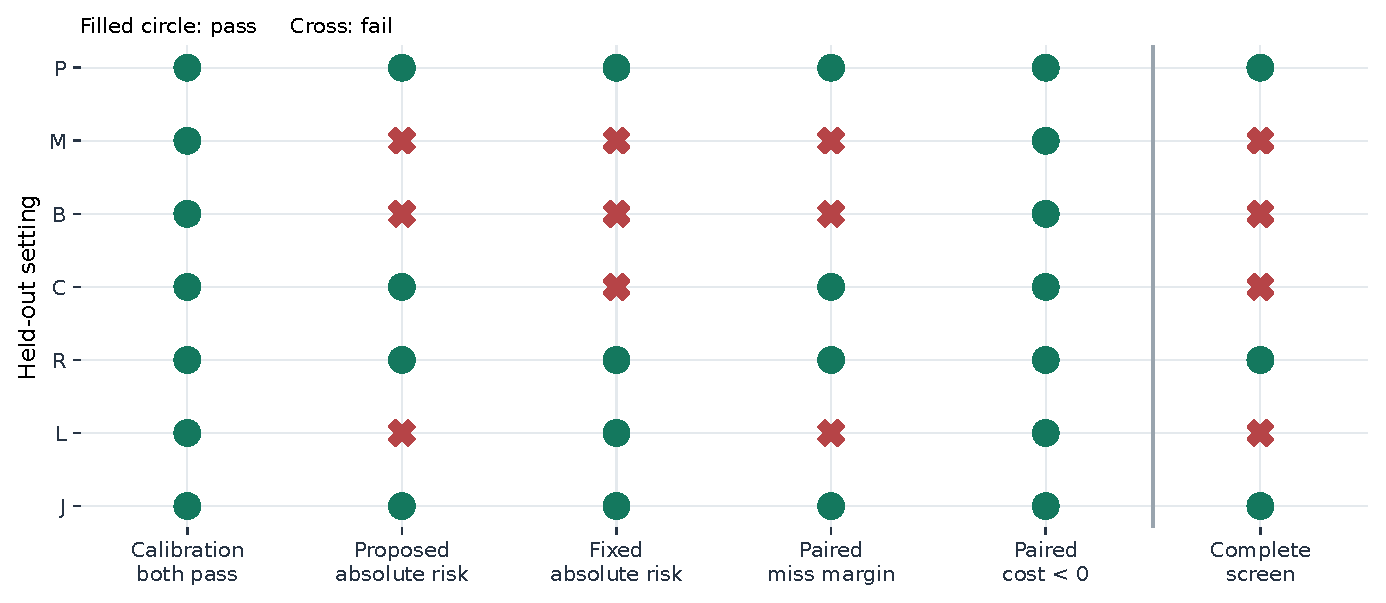
\includegraphics[width=.98\linewidth]{screen_matrix.pdf}
\caption{Qualification of proposed versus fixed capacity, decomposed by condition.}
\label{fig:screen}\end{figure*}
\begin{table*}[htbp]\centering\footnotesize
\caption{Common-target comparison against fixed capacity. Upper endpoints are percentages. Cost intervals are paired, unadjusted 95\% intervals.}
\begin{tabular}{lccrl}\toprule Setting & Proposed $(U_0,U_1)$ & Fixed $(U_0,U_1)$ & $\Delta J$ [95\% interval] & Qualified\\\midrule
P & (0.0000, 0.0000) & (0.0000, 0.0457) & -2520.2 [-2593.1, -2447.0] & Yes \\
M & (0.2485, 1.9804) & (0.0173, 2.4488) & -2180.8 [-2448.9, -1889.4] & No \\
B & (0.6058, 0.2601) & (0.2013, 0.7197) & -1402.7 [-1917.4, -844.9] & No \\
C & (0.0000, 0.0000) & (0.0000, 0.1349) & -2506.4 [-2584.6, -2425.6] & No \\
R & (0.0331, 0.0000) & (0.0000, 0.0789) & -2478.2 [-2577.8, -2378.0] & Yes \\
L & (1.1927, 9.8982) & (0.0000, 0.0623) & -2156.4 [-2227.3, -2082.4] & No \\
J & (0.0000, 0.0062) & (0.0140, 0.0581) & -2378.9 [-2463.9, -2286.0] & Yes \\
\bottomrule\end{tabular}\label{tab:qualified}
\end{table*}
Table~\ref{tab:qualified} supplies the endpoints behind that decision. In P,
mean cost is 4159.85 versus 6680.00 for fixed provisioning. The paired difference
is $-2520.15$, with a 95\% interval approximately $[-2593.1,-2447.0]$.
Qualified savings are 37.73\% in P, 37.10\% in R and 35.61\% in J.
Figure~\ref{fig:qualified} shows why negative cost differences in the other
settings must remain unqualified. These comparisons use common thresholds,
not proof that the policies have identical underlying reliability.
\begin{figure*}[htbp]\centering
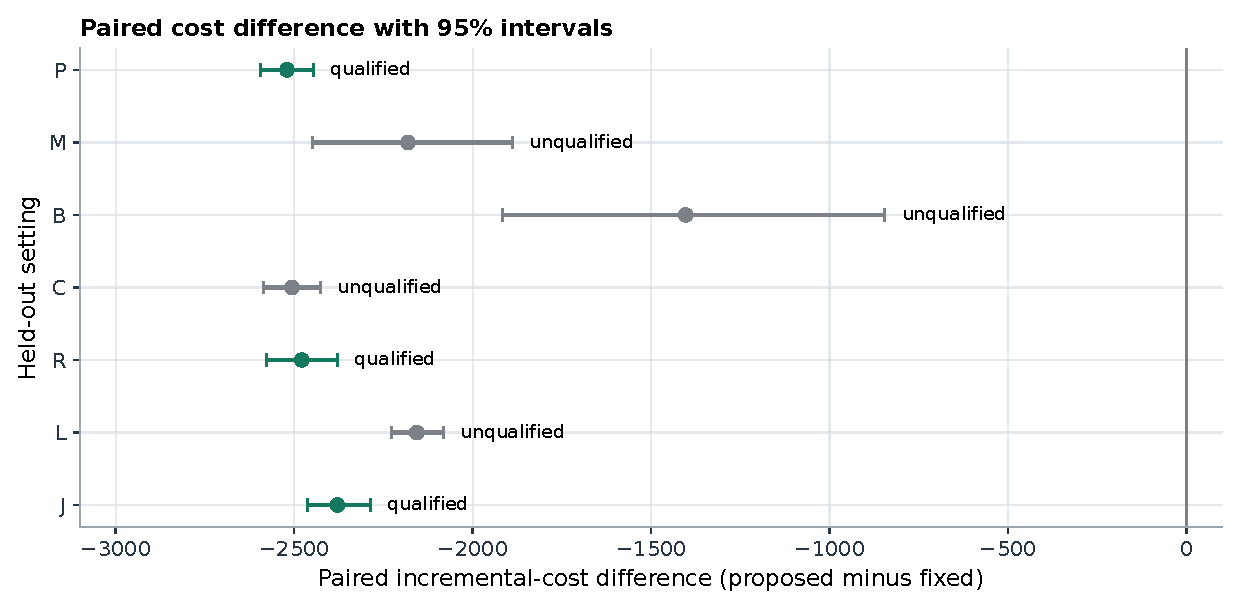
\includegraphics[width=.94\linewidth]{qualified_cost.pdf}
\caption{Paired cost differences, proposed minus fixed. Green denotes a
comparison satisfying the entire descriptive qualification rule. Gray denotes
an unqualified comparison, regardless of the direction of its cost difference.
Intervals are unadjusted 95\% paired-bootstrap intervals.}
\label{fig:qualified}
\end{figure*}

Figure~\ref{fig:primary} separates resource cost from each class's miss fraction.
Under Markov traffic M, proposed mean misses are 0.0915\% and 0.8811\%.
Under compound batches B, they are 0.3413\% and 0.1297\%. Their upper endpoints
fail the target. Mean-matched burst states therefore do not preserve the
periodic calibration result. Both the duration of unfavorable service periods
and the arrival process seen by each queue matter.
\begin{figure*}[htbp]\centering
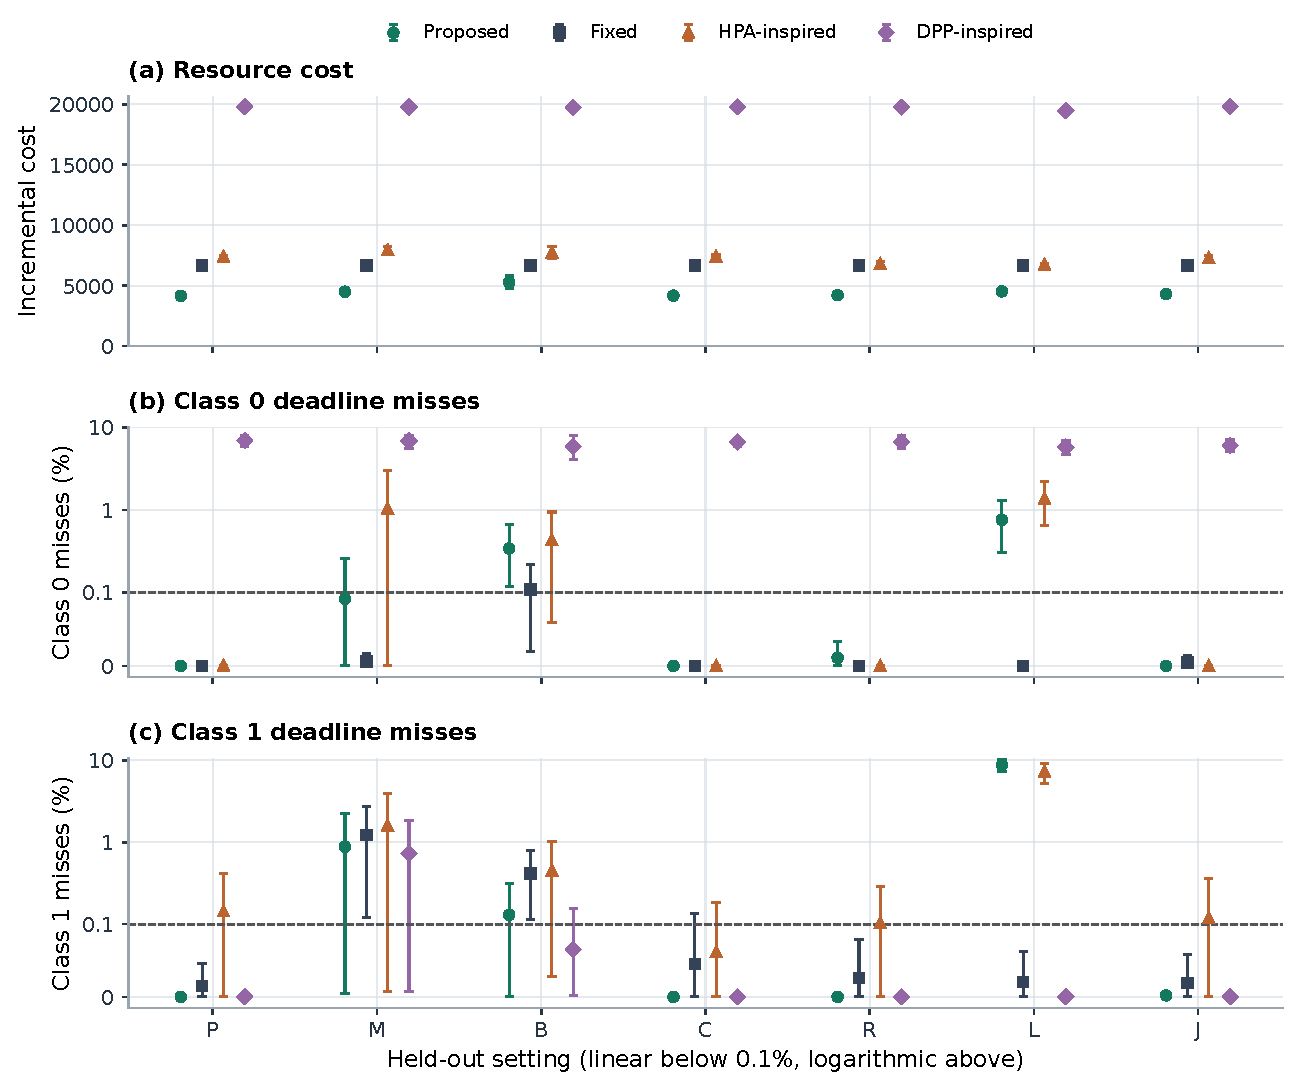
\includegraphics[width=.98\linewidth]{reliability_primary.pdf}
\caption{Held-out costs and deadline-miss percentages with unadjusted 95\%
seed-bootstrap intervals. P, M, B, C, R, L and J are defined in
Table~\ref{tab:settings}. The 0.1\% dashed line is the common target.
The DPP-inspired adaptation is calibration-ineligible and diagnostic only.}
\label{fig:primary}
\end{figure*}
For batch size $b=3$, conditional arrivals are $A_s=bK_s$ with
$K_s\sim\operatorname{Poisson}(\lambda_s/b)$. Hence
\begin{equation}
 \mathbb E[A_s\mid\lambda_s]=\lambda_s,\qquad
 \operatorname{Var}(A_s\mid\lambda_s)=b\lambda_s.
 \label{eq:batchmoments}
\end{equation}
The compound case changes dispersion without changing conditional mean.
However, the reported $v_{is}$ measures net ingress minus service, not arrival
variance alone. Reservations and borrowing also change with the resulting
queue trajectories. The opposite movements of the two class means between M
and B therefore cannot be summarized as a monotone classwise variance effect.

In L, $L=50$ exceeds both deadlines, and class-1 mean misses reach 8.7846\%
versus 0.0208\% for fixed provisioning. For any packet already present at issue, $\omega_{sa}\le0$ because $L>D_s$. Its current command therefore cannot change an on-time completion. The irreversibility property explains
the timing obstruction: a new command cannot change service before activation.
The horizon mismatch in \eqref{eq:scoreerror} provides an additional reason
not to interpret a bounded dispersion term as protection against this delay.
J instead mixes shorter and longer delays, has mean 18.2 slots, and announces
each delay on issue. Its successful screen neither contradicts L nor isolates
the effect of jitter at equal mean delay.


Figure~\ref{fig:ablation} compares the proposed controller with a rate-only
projection at the same headroom and with an uncalibrated ledger variant.
In P, the no-ledger cost is 4619.93 versus 4159.85 for the proposed policy,
approximately a 9.96\% reduction. Both have zero observed misses. The
uncalibrated controller is cheaper at 2737.40, but its class means become
0.0570\% and 0.1447\%. The two ablations answer different questions:
ledger availability at fixed headroom, and headroom selection with the ledger
present. Their effects should not be merged into one causal attribution.
\begin{figure*}[htbp]\centering
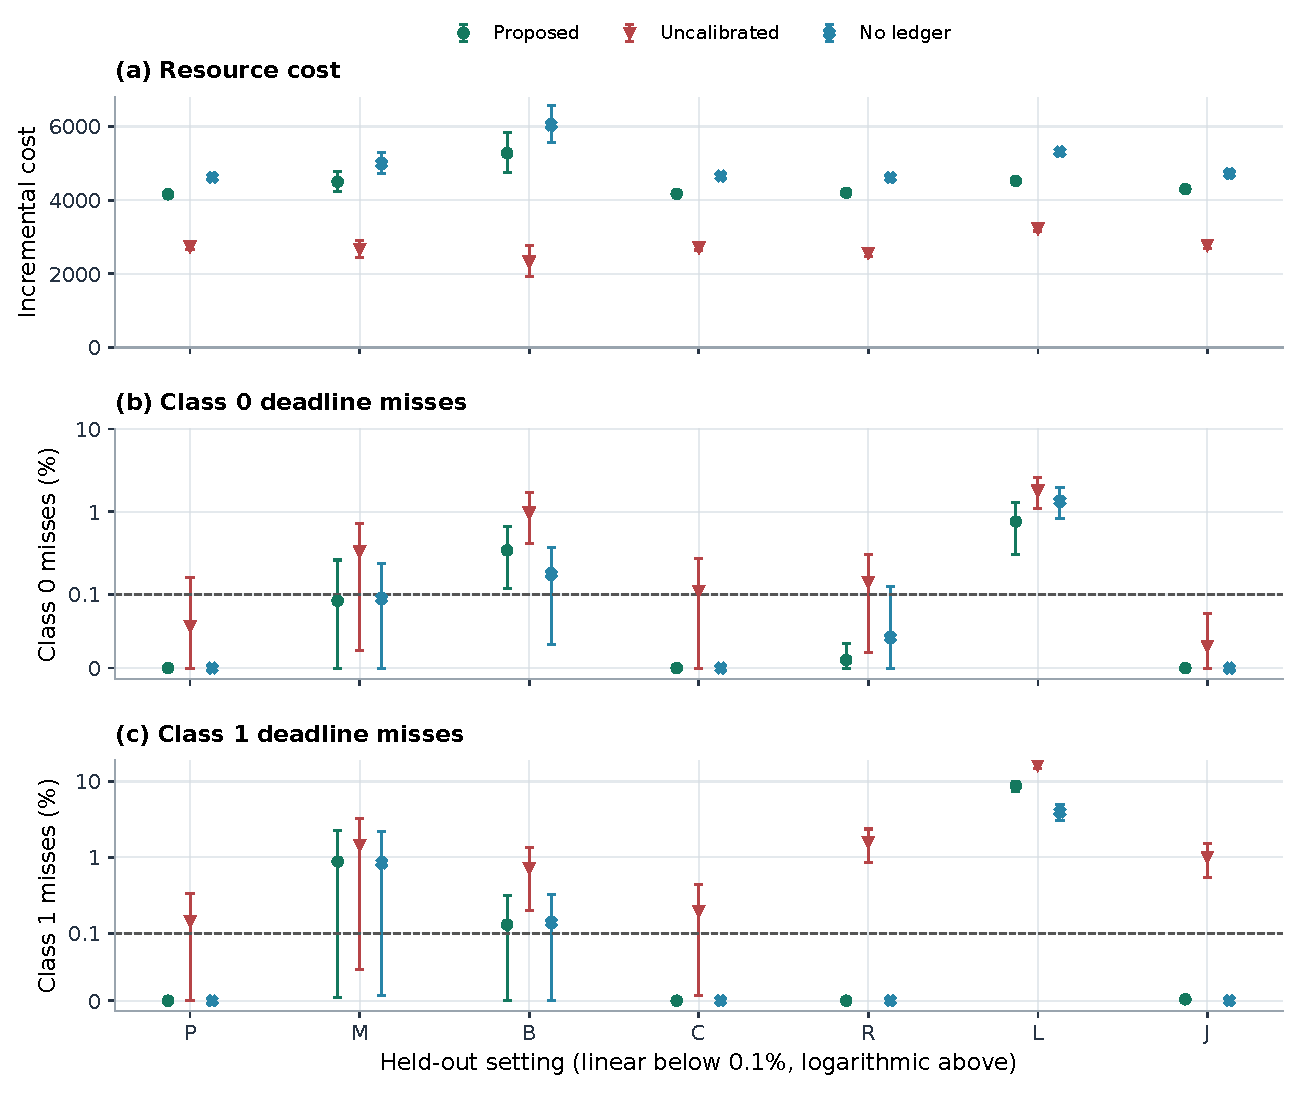
\includegraphics[width=.96\linewidth]{reliability_ablation.pdf}
\caption{Component ablations on identical test seeds. The uncalibrated controller
uses $\eta=1$. The no-ledger controller retains selected headroom but uses a
drift projection. The error bars describe seed-mean uncertainty, not predictive
confidence bounds for the controller.}
\label{fig:ablation}
\end{figure*}
To connect these cost differences to the objective, write
\begin{equation}
\begin{aligned}
 J&=J_{\mathrm{cap}}+J_{\mathrm{sw}},\qquad J_{\mathrm{cap}}=\sum_{t,i}e_i(t),\\
 J_{\mathrm{sw}}&=\kappa\sum_{a\in\mathcal A_T}\|x_a-e_a^-\|_1.
\end{aligned}
\label{eq:costdecomposition}
\end{equation}
Figure~\ref{fig:components} recomputes these terms from the saved per-run
counters. The hatched caps in panel (a) show switching, enlarged separately
in panel (b). They are not additional experiments or newly selected outcomes.

In P, the ledger variant has mean capacity cost 4100.75
and switching cost 59.10. The no-ledger values are
4551.25 and 68.675.
The capacity difference is 450.50, accounting for
97.92\% of the total mean cost difference. Thus the nominal saving is
primarily reduced active capacity, not merely reduced switching charges.

\begin{figure*}[!htbp]\centering
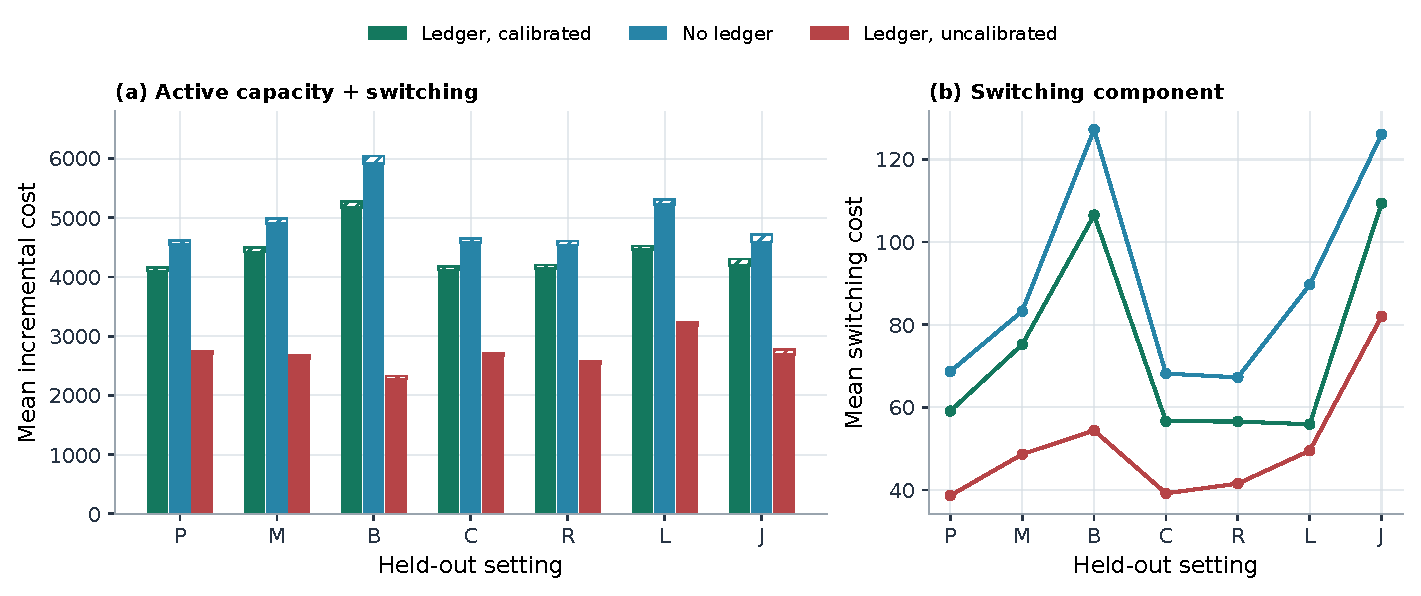
\includegraphics[width=.85\linewidth]{cost_components.pdf}
\caption{Post hoc cost decomposition of the frozen ablation runs. Hatched caps denote switching cost.}
\label{fig:components}\end{figure*}
\begin{figure*}[!htbp]\centering
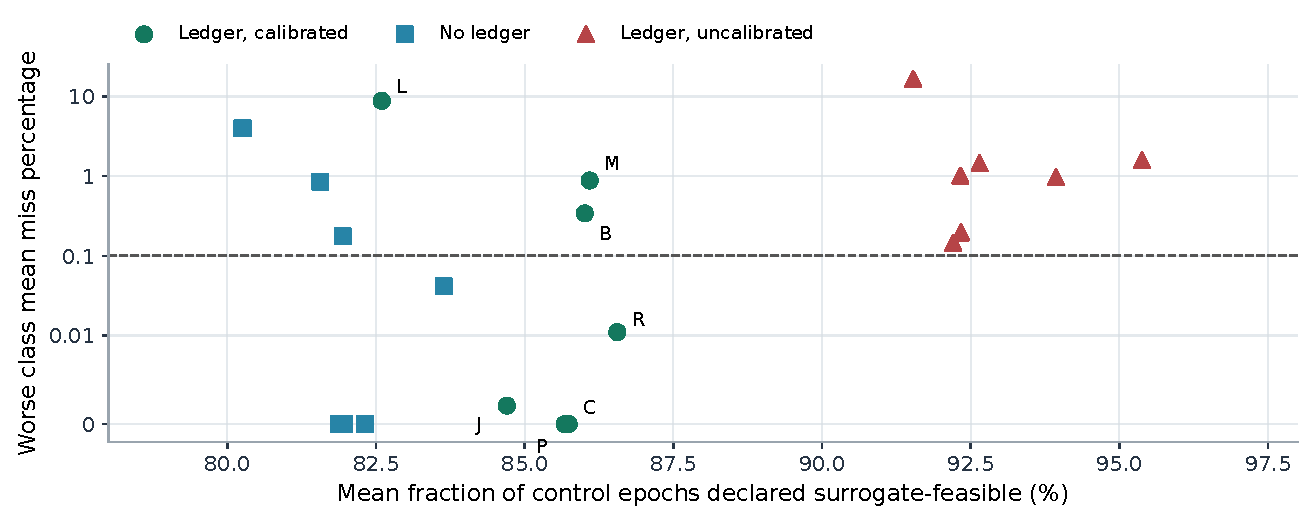
\includegraphics[width=.85\linewidth]{proxy_vs_outcome.pdf}
\caption{Post hoc proxy--outcome diagnostic. Labels identify proposed-policy settings. The dashed line is 0.1\%.}
\label{fig:proxyoutcome}\end{figure*}
The ledger is not uniformly beneficial to deadlines. In L, its class-1 mean
miss fraction is 8.7846\% compared with 3.9807\% without the ledger. Neither
passes the absolute screen, and the ledger uses less capacity. This is a
cost--risk trade-off, not evidence that the ledger is always preferable.
The aggregate counters also do not measure forecast error or explain the
timing of every capacity release. Such mechanisms require per-slot traces.



Define the run-level feasible-decision frequency
\begin{equation}
 \phi=\frac1{N_{\mathrm{ctrl}}}\sum_{t\in\mathcal T_{\mathrm{ctrl}}}
 \mathbf 1\{\max_s\rho_s(x_t,\alpha_t)\le1\},
 \label{eq:feasiblefrequency}
\end{equation}
where $\mathcal T_{\mathrm{ctrl}}$ is the set of control epochs and
$N_{\mathrm{ctrl}}$ its size. Figure~\ref{fig:proxyoutcome} compares the
seed-mean $\phi$ with the worse of the two class seed-mean miss fractions.
This exploratory diagnostic uses existing counters. It is not a calibration
criterion, a prediction-accuracy test, or an event-level correlation analysis.

The proposed controller declares 85.67\%
of decisions feasible in P and 86.09\%
in M, although the worse class mean changes from zero to
0.8811\%.
In L, 82.60\% of decisions remain
surrogate-feasible while the worse class mean reaches
8.7846\%.

Equations~\eqref{eq:structuralslack}--\eqref{eq:slackbound} explain why a positive queue-level margin does not reveal recoverable deadline slack. Likewise, \eqref{eq:demanderror}--\eqref{eq:scoreerror} show that a nominal $\rho_s\le1$ leaves demand-error exposure unbudgeted. The proxy does not encode packet ages, coupled downstream forecasts or an
error budget over the full activation horizon. Consequently, similar values
of $\phi$ can coexist with very different deadline outcomes. Smaller headroom
tightens the score, but it does not repair those omitted state variables.




\section{Discussion and Deployment Boundary}
The supported advantage is conditional. P and R test repeatability within
the calibration traffic constructions, while J tests one announced-delay
law. Failures in M, B and L prevent extrapolation to general workload or
latency robustness. Integer reservations, headroom and ledger replay explain
how decisions are formed. Their consistency with aggregate results does not
identify forecast accuracy or establish packet-level guarantees.

Six seeds per calibration stratum, twenty per test setting, all-zero samples
and unadjusted comparisons limit inference at the 0.1\% target. The fixed
reference has its own share policy, and HPA/DPP are adaptations. Neither
competitive-system reproduction nor physical O-RAN validation is provided.
The next validation steps are measured service and interface-delay mappings,
recorded workloads, independently implemented baselines and larger reliability
experiments. Channel variation, retransmissions and virtualization interference
must enter that model before interpreting abstract cost as deployment benefit.

\section{Conclusion}
The action-ledger controller separates measured, requested and activated
capacity. With independently calibrated headroom, it yields qualified cost
reductions of 35.61--37.73\% against fixed provisioning in three of seven
synthetic settings. Its nominal ledger ablation saves approximately 9.96\%,
primarily through lower active capacity, with zero observed misses for both
variants. Shifted traffic and long actuation nevertheless expose deadline
failures despite frequent surrogate-feasible decisions. The resulting
contribution is an auditable controller and a reproducible boundary on its
empirical benefit, not a deadline certificate or demonstrated superiority
over deployed O-RAN systems.

\clearpage
\onecolumn
\appendices
\section{Complete Held-Out Results}
Table~\ref{tab:allresults} reports every method and setting using the same classwise metrics.

\begin{table}[!htbp]\centering\fontsize{8}{9}\selectfont\renewcommand{\arraystretch}{1.06}
\caption{Complete test results, twenty seeds per row. Miss fractions and one-sided upper endpoints are percentages. DPP-inspired results are diagnostic after calibration failure.}\label{tab:allresults}
\begin{tabular}{llrrrrr}
\toprule Setting & Method & Mean $V_0$ & Mean $V_1$ & Upper $V_0$ & Upper $V_1$ & Mean cost\\\midrule
P & Proposed & 0.0000 & 0.0000 & 0.0000 & 0.0000 & 4159.85 \\
P & Fixed & 0.0000 & 0.0152 & 0.0000 & 0.0457 & 6680.00 \\
P & HPA-inspired & 0.0000 & 0.1436 & 0.0000 & 0.3977 & 7400.26 \\
P & DPP-inspired & 6.9240 & 0.0000 & 7.7209 & 0.0000 & 19805.75 \\
P & Uncalibrated & 0.0570 & 0.1447 & 0.1463 & 0.2973 & 2737.40 \\
P & No ledger & 0.0000 & 0.0000 & 0.0000 & 0.0000 & 4619.93 \\
\addlinespace
M & Proposed & 0.0915 & 0.8811 & 0.2485 & 1.9804 & 4499.21 \\
M & Fixed & 0.0058 & 1.2169 & 0.0173 & 2.4488 & 6680.00 \\
M & HPA-inspired & 1.0388 & 1.6008 & 2.9262 & 3.5819 & 7932.65 \\
M & DPP-inspired & 6.8437 & 0.7340 & 7.8499 & 1.5975 & 19779.96 \\
M & Uncalibrated & 0.3303 & 1.4469 & 0.6362 & 2.9848 & 2671.89 \\
M & No ledger & 0.0942 & 0.8468 & 0.2135 & 1.8537 & 4992.29 \\
\addlinespace
B & Proposed & 0.3413 & 0.1297 & 0.6058 & 0.2601 & 5277.30 \\
B & Fixed & 0.1084 & 0.4146 & 0.2013 & 0.7197 & 6680.00 \\
B & HPA-inspired & 0.4319 & 0.4528 & 0.8366 & 0.9144 & 7729.49 \\
B & DPP-inspired & 5.8678 & 0.0652 & 7.5206 & 0.1349 & 19738.71 \\
B & Uncalibrated & 0.9710 & 0.7176 & 1.5660 & 1.2352 & 2329.66 \\
B & No ledger & 0.1766 & 0.1378 & 0.3322 & 0.2777 & 6044.76 \\
\addlinespace
C & Proposed & 0.0000 & 0.0000 & 0.0000 & 0.0000 & 4173.62 \\
C & Fixed & 0.0000 & 0.0450 & 0.0000 & 0.1349 & 6680.00 \\
C & HPA-inspired & 0.0000 & 0.0618 & 0.0000 & 0.1853 & 7388.18 \\
C & DPP-inspired & 6.6611 & 0.0000 & 7.3007 & 0.0000 & 19790.64 \\
C & Uncalibrated & 0.1099 & 0.1963 & 0.2439 & 0.4068 & 2715.18 \\
C & No ledger & 0.0000 & 0.0000 & 0.0000 & 0.0000 & 4653.68 \\
\addlinespace
R & Proposed & 0.0110 & 0.0000 & 0.0331 & 0.0000 & 4201.81 \\
R & Fixed & 0.0000 & 0.0263 & 0.0000 & 0.0789 & 6680.00 \\
R & HPA-inspired & 0.0000 & 0.1031 & 0.0000 & 0.2656 & 6814.40 \\
R & DPP-inspired & 6.6940 & 0.0000 & 7.7193 & 0.0000 & 19766.59 \\
R & Uncalibrated & 0.1412 & 1.5900 & 0.2721 & 2.2523 & 2569.54 \\
R & No ledger & 0.0414 & 0.0000 & 0.1243 & 0.0000 & 4609.25 \\
\addlinespace
L & Proposed & 0.7593 & 8.7846 & 1.1927 & 9.8982 & 4523.64 \\
L & Fixed & 0.0000 & 0.0208 & 0.0000 & 0.0623 & 6680.00 \\
L & HPA-inspired & 1.3767 & 7.2461 & 2.0694 & 8.8912 & 6731.15 \\
L & DPP-inspired & 5.7789 & 0.0000 & 6.6497 & 0.0000 & 19461.90 \\
L & Uncalibrated & 1.7900 & 16.4355 & 2.4647 & 17.7445 & 3226.75 \\
L & No ledger & 1.3369 & 3.9807 & 1.8522 & 4.8110 & 5314.18 \\
\addlinespace
J & Proposed & 0.0000 & 0.0021 & 0.0000 & 0.0062 & 4301.07 \\
J & Fixed & 0.0047 & 0.0194 & 0.0140 & 0.0581 & 6680.00 \\
J & HPA-inspired & 0.0000 & 0.1194 & 0.0000 & 0.3582 & 7312.54 \\
J & DPP-inspired & 6.0246 & 0.0000 & 6.8568 & 0.0000 & 19819.75 \\
J & Uncalibrated & 0.0302 & 1.0178 & 0.0636 & 1.4476 & 2776.40 \\
J & No ledger & 0.0000 & 0.0000 & 0.0000 & 0.0000 & 4716.75 \\
\addlinespace
\bottomrule\end{tabular}\end{table}
\clearpage
\section{Complete Paired Comparisons}
Table~\ref{tab:allpaired} reports cost and miss differences for every comparator.

\begin{table}[!htbp]\centering\fontsize{8}{9}\selectfont\renewcommand{\arraystretch}{1.06}
\caption{All paired contrasts, proposed minus comparator. Miss differences and upper endpoints are percentage points. No multiplicity-adjusted claim is made.}\label{tab:allpaired}
\begin{tabular}{llrcc}
\toprule Setting & Comparator & $\Delta J$ [95\% interval] & Mean $(\Delta V_0,\Delta V_1)$ & Upper $(\Delta V_0,\Delta V_1)$\\\midrule
P & Fixed & -2520.2 [-2593.1, -2447.0] & (0.0000, -0.0152) & (0.0000, 0.0000) \\
P & HPA-inspired & -3240.4 [-3351.1, -3130.5] & (0.0000, -0.1436) & (0.0000, 0.0000) \\
P & DPP-inspired & -15645.9 [-15721.6, -15569.6] & (-6.9240, 0.0000) & (-6.1061, 0.0000) \\
P & Uncalibrated & 1422.5 [1357.5, 1490.1] & (-0.0570, -0.1447) & (0.0000, -0.0284) \\
P & No ledger & -460.1 [-510.0, -410.2] & (0.0000, 0.0000) & (0.0000, 0.0000) \\
\addlinespace
M & Fixed & -2180.8 [-2448.9, -1889.4] & (0.0857, -0.3358) & (0.2312, -0.1143) \\
M & HPA-inspired & -3433.4 [-3647.5, -3181.9] & (-0.9473, -0.7197) & (0.0015, 0.0200) \\
M & DPP-inspired & -15280.8 [-15559.1, -14975.8] & (-6.7522, 0.1471) & (-5.7626, 0.3231) \\
M & Uncalibrated & 1827.3 [1718.1, 1944.4] & (-0.2388, -0.5658) & (-0.0195, -0.0159) \\
M & No ledger & -493.1 [-586.8, -403.3] & (-0.0028, 0.0344) & (0.0924, 0.1165) \\
\addlinespace
B & Fixed & -1402.7 [-1917.4, -844.9] & (0.2329, -0.2850) & (0.4310, -0.1079) \\
B & HPA-inspired & -2452.2 [-2614.5, -2295.6] & (-0.0905, -0.3231) & (0.0997, -0.0685) \\
B & DPP-inspired & -14461.4 [-14977.8, -13899.2] & (-5.5265, 0.0645) & (-4.1229, 0.1515) \\
B & Uncalibrated & 2947.6 [2710.2, 3175.2] & (-0.6297, -0.5879) & (-0.2582, -0.2014) \\
B & No ledger & -767.5 [-839.8, -690.4] & (0.1647, -0.0081) & (0.3303, 0.0000) \\
\addlinespace
C & Fixed & -2506.4 [-2584.6, -2425.6] & (0.0000, -0.0450) & (0.0000, 0.0000) \\
C & HPA-inspired & -3214.6 [-3358.2, -3071.5] & (0.0000, -0.0618) & (0.0000, 0.0000) \\
C & DPP-inspired & -15617.0 [-15710.2, -15526.1] & (-6.6611, 0.0000) & (-5.9980, 0.0000) \\
C & Uncalibrated & 1458.5 [1393.4, 1520.2] & (-0.1099, -0.1963) & (-0.0062, -0.0326) \\
C & No ledger & -480.1 [-544.8, -417.0] & (0.0000, 0.0000) & (0.0000, 0.0000) \\
\addlinespace
R & Fixed & -2478.2 [-2577.8, -2378.0] & (0.0110, -0.0263) & (0.0331, 0.0000) \\
R & HPA-inspired & -2612.6 [-2782.0, -2432.3] & (0.0110, -0.1031) & (0.0331, 0.0000) \\
R & DPP-inspired & -15564.8 [-15669.4, -15463.9] & (-6.6830, 0.0000) & (-5.6565, 0.0000) \\
R & Uncalibrated & 1632.3 [1541.1, 1726.6] & (-0.1302, -1.5900) & (-0.0172, -0.9720) \\
R & No ledger & -407.4 [-476.0, -341.8] & (-0.0304, 0.0000) & (0.0221, 0.0000) \\
\addlinespace
L & Fixed & -2156.4 [-2227.3, -2082.4] & (0.7593, 8.7638) & (1.1927, 9.8689) \\
L & HPA-inspired & -2207.5 [-2330.2, -2083.7] & (-0.6174, 1.5385) & (0.0462, 3.0453) \\
L & DPP-inspired & -14938.3 [-15000.8, -14871.3] & (-5.0197, 8.7846) & (-4.2307, 9.8982) \\
L & Uncalibrated & 1296.9 [1217.8, 1376.6] & (-1.0308, -7.6509) & (-0.5847, -6.6234) \\
L & No ledger & -790.5 [-874.8, -698.8] & (-0.5776, 4.8039) & (-0.0554, 5.5754) \\
\addlinespace
J & Fixed & -2378.9 [-2463.9, -2286.0] & (-0.0047, -0.0173) & (0.0000, 0.0000) \\
J & HPA-inspired & -3011.5 [-3146.5, -2883.1] & (0.0000, -0.1173) & (0.0000, 0.0042) \\
J & DPP-inspired & -15518.7 [-15624.6, -15403.8] & (-6.0246, 0.0021) & (-5.2649, 0.0062) \\
J & Uncalibrated & 1524.7 [1446.8, 1604.0] & (-0.0302, -1.0158) & (0.0000, -0.6151) \\
J & No ledger & -415.7 [-478.1, -355.4] & (0.0000, 0.0021) & (0.0000, 0.0062) \\
\addlinespace
\bottomrule\end{tabular}\end{table}

\clearpage\twocolumn
\section{Reproduction Contract}
Run \texttt{python reliability\_study.py} to reproduce the calibration and
held-out matrix. Existing complete checkpoints are reused only if the frozen
protocol hash matches. Remove or relocate those specific checkpoint files
to execute all runs anew. Run \texttt{python verify\_reliability.py} to reconcile
all metrics and selected deterministic replays, followed by
\texttt{python build\_reliability\_paper.py} and
\texttt{python build\_release.py}. The archive includes the exact dependency
versions and checksums. The PDF is generated from saved results, not from
hand-entered headline numbers. Reproduction establishes consistency of this
synthetic experiment, not external validity for a physical network.


\section*{Data and Code Availability}
The archive provides code, the frozen protocol, all 1176 execution records,
verification tests, manuscript sources and vector figures. Additional
diagnostics reuse those records. Historical studies remain separate. No
external dataset is used. The code, frozen execution records and reproduction instructions are available at \href{https://github.com/YassirALKarawi/oran-telemetry-elasticity}{github.com/YassirALKarawi/oran-telemetry-elasticity}.


\small\begin{thebibliography}{99}\setlength{\itemsep}{2pt}
\bibitem{polese} M. Polese et al., ``Understanding O-RAN: Architecture, Interfaces, Algorithms, Security, and Research Challenges,'' IEEE Communications Surveys \& Tutorials, vol. 25, no. 2, pp. 1376--1411, 2023. \href{https://doi.org/10.1109/COMST.2023.3239220}{10.1109/COMST.2023.3239220}.
\bibitem{sdn} D. Kreutz et al., ``Software-Defined Networking: A Comprehensive Survey,'' Proceedings of the IEEE, vol. 103, no. 1, pp. 14--76, 2015. \href{https://doi.org/10.1109/JPROC.2014.2371999}{10.1109/JPROC.2014.2371999}.
\bibitem{ecosystem} A. Garcia-Saavedra and X. Costa-Perez, ``O-RAN: Disrupting the Virtualized RAN Ecosystem,'' IEEE Communications Standards Magazine, vol. 5, no. 4, pp. 96--103, 2021. \href{https://doi.org/10.1109/MCOMSTD.101.2000014}{10.1109/MCOMSTD.101.2000014}.
\bibitem{age} R. D. Yates et al., ``Age of Information: An Introduction and Survey,'' IEEE Journal on Selected Areas in Communications, vol. 39, no. 5, pp. 1183--1210, 2021. \href{https://doi.org/10.1109/JSAC.2021.3065072}{10.1109/JSAC.2021.3065072}.
\bibitem{networked} J. P. Hespanha, P. Naghshtabrizi, and Y. Xu, ``A Survey of Recent Results in Networked Control Systems,'' Proceedings of the IEEE, vol. 95, no. 1, pp. 138--162, 2007. \href{https://doi.org/10.1109/JPROC.2006.887288}{10.1109/JPROC.2006.887288}.
\bibitem{mpc} D. Q. Mayne, J. B. Rawlings, C. V. Rao, and P. O. M. Scokaert, ``Constrained model predictive control: Stability and optimality,'' Automatica, vol. 36, no. 6, pp. 789--814, 2000. \href{https://doi.org/10.1016/S0005-1098(99)00214-9}{10.1016/S0005-1098(99)00214-9}.
\bibitem{orchestr} S. D'Oro, L. Bonati, M. Polese, and T. Melodia, ``OrchestRAN: Network Automation through Orchestrated Intelligence in the Open RAN,'' IEEE INFOCOM, 2022, author version arXiv:2201.05632. \href{https://doi.org/10.48550/arXiv.2201.05632}{10.48550/arXiv.2201.05632}.
\bibitem{oreo} F. Mungari, C. Puligheddu, A. Garcia-Saavedra, and C. F. Chiasserini, ``O-RAN Intelligence Orchestration Framework for Quality-Driven xApp Deployment and Sharing,'' IEEE Transactions on Mobile Computing, vol. 24, no. 6, pp. 4811--4828, 2025. \href{https://doi.org/10.1109/TMC.2025.3527707}{10.1109/TMC.2025.3527707}.
\bibitem{demir} O. T. Demir, M. Masoudi, E. Bjornson, and C. Cavdar, ``Cell-Free Massive MIMO in O-RAN: Energy-Aware Joint Orchestration of Cloud, Fronthaul, and Radio Resources,'' IEEE Journal on Selected Areas in Communications, vol. 42, no. 2, pp. 356--372, 2024. \href{https://doi.org/10.1109/JSAC.2023.3336187}{10.1109/JSAC.2023.3336187}.
\bibitem{vrain} J. A. Ayala-Romero et al., ``vrAIn: A Deep Learning Approach Tailoring Computing and Radio Resources in Virtualized RANs,'' ACM MobiCom, 2019. \href{https://doi.org/10.1145/3300061.3345431}{10.1145/3300061.3345431}.
\bibitem{nuberu} G. Garcia-Aviles et al., ``Nuberu: Reliable RAN virtualization in shared platforms,'' ACM MobiCom, 2021. \href{https://doi.org/10.1145/3447993.3483266}{10.1145/3447993.3483266}.
\bibitem{concordia} X. Foukas and B. Radunovic, ``Concordia: Teaching the 5G vRAN to Share Compute,'' ACM SIGCOMM, 2021. \href{https://www.microsoft.com/en-us/research/publication/concordia-teaching-the-5g-vran-to-share-compute/}{Author/publisher source}.
\bibitem{kalntis} M. Kalntis, G. Iosifidis, and F. A. Kuipers, ``Adaptive Resource Allocation for Virtualized Base Stations in O-RAN With Online Learning,'' IEEE Transactions on Communications, vol. 73, no. 3, pp. 1787--1800, 2025. \href{https://doi.org/10.1109/TCOMM.2024.3461569}{10.1109/TCOMM.2024.3461569}.
\bibitem{marea} O. Adamuz-Hinojosa, L. Zanzi, V. Sciancalepore, and X. Costa-Perez, ``MAREA: A Delay-Aware Multi-Time-Scale Radio Resource Orchestrator for 6G O-RAN,'' IEEE Transactions on Communications, vol. 73, no. 9, pp. 7695--7710, 2025. \href{https://doi.org/10.1109/TCOMM.2025.3552296}{10.1109/TCOMM.2025.3552296}.
\bibitem{caora} S. D. A. Shah, M. Hafeez, A. Salama, and S. A. R. Zaidi, ``Proactive AI-and-RAN Workload Orchestration in O-RAN Architectures for 6G Networks,'' author version, arXiv:2507.09124, 2025. \href{https://doi.org/10.48550/arXiv.2507.09124}{10.48550/arXiv.2507.09124}.
\bibitem{murti} F. W. Murti, S. Ali, G. Iosifidis, and M. Latva-aho, ``Learning-Based Orchestration for Dynamic Functional Split and Resource Allocation in vRANs,'' EuCNC/6G Summit, 2022. \href{https://doi.org/10.1109/EuCNC/6GSummit54941.2022.9815815}{10.1109/EuCNC/6GSummit54941.2022.9815815}.
\bibitem{wang} Q. Wang et al., ``Resource Allocation Based on Radio Intelligence Controller for Open RAN Toward 6G,'' IEEE Access, vol. 11, pp. 97909--97919, 2023. \href{https://doi.org/10.1109/ACCESS.2023.3311888}{10.1109/ACCESS.2023.3311888}.
\bibitem{kasuluru} V. Kasuluru et al., ``Cloud-Native Multivariate Probabilistic Forecasting for Next-Generation Resource Allocation in O-RAN,'' IEEE Access, vol. 14, pp. 2904--2923, 2026. \href{https://doi.org/10.1109/ACCESS.2025.3648065}{10.1109/ACCESS.2025.3648065}.
\bibitem{sora} A. Tuerxun and A. Nakao, ``SORA: Energy-Efficient Resource Allocation in Open Radio Access Network With Online Learning,'' IEEE Access, vol. 13, pp. 113686--113701, 2025. \href{https://doi.org/10.1109/ACCESS.2025.3584345}{10.1109/ACCESS.2025.3584345}.
\bibitem{comix} A. E. Giannopoulos et al., ``COMIX: Generalized Conflict Management in O-RAN xApps---Architecture, Workflow, and a Power Control Case,'' IEEE Access, vol. 13, pp. 116684--116700, 2025. \href{https://doi.org/10.1109/ACCESS.2025.3585774}{10.1109/ACCESS.2025.3585774}.
\bibitem{5erasi} M. Iqbal and A. Nakao, ``5ERASI: 5G Service-Enabled Resource Allocation and Sub-Slice Isolation for Open RAN,'' IEEE Access, 2026. \href{https://doi.org/10.1109/ACCESS.2026.3693783}{10.1109/ACCESS.2026.3693783}.
\bibitem{radiosaber} Y. Chen, R. Yao, H. Hassanieh, and R. Mittal, ``Channel-Aware 5G RAN Slicing with Customizable Schedulers,'' USENIX NSDI, pp. 1767--1782, 2023. \href{https://www.usenix.org/conference/nsdi23/presentation/chen-yongzhou}{Author/publisher source}.
\bibitem{edgeric} W.-H. Ko et al., ``EdgeRIC: Empowering Real-time Intelligent Optimization and Control in NextG Cellular Networks,'' USENIX NSDI, pp. 1315--1330, 2024. \href{https://www.usenix.org/conference/nsdi24/presentation/ko}{Author/publisher source}.
\bibitem{coloran} M. Polese, L. Bonati, S. D'Oro, S. Basagni, and T. Melodia, ``ColO-RAN: Developing Machine Learning-based xApps for Open RAN Closed-loop Control on Programmable Experimental Platforms,'' IEEE Transactions on Mobile Computing, vol. 22, no. 10, pp. 5787--5800, 2023. \href{https://doi.org/10.1109/TMC.2022.3188013}{10.1109/TMC.2022.3188013}.
\bibitem{gym} L. Bonati, M. Polese, S. D'Oro, S. Basagni, and T. Melodia, ``OpenRAN Gym: AI/ML Development, Data Collection, and Testing for O-RAN on PAWR Platforms,'' Computer Networks, vol. 220, article 109502, 2023. \href{https://doi.org/10.1016/j.comnet.2022.109502}{10.1016/j.comnet.2022.109502}.
\bibitem{scope} L. Bonati, S. D'Oro, S. Basagni, and T. Melodia, ``SCOPE: An Open and Softwarized Prototyping Platform for NextG Systems,'' ACM MobiSys, 2021. \href{https://doi.org/10.1145/3458864.3466863}{10.1145/3458864.3466863}.
\bibitem{flexric} R. Schmidt, M. Irazabal, and N. Nikaein, ``FlexRIC: an SDK for next-generation SD-RANs,'' ACM CoNEXT, pp. 411--425, 2021. \href{https://doi.org/10.1145/3485983.3494870}{10.1145/3485983.3494870}.
\bibitem{nsoran} A. Lacava et al., ``ns-O-RAN: Simulating O-RAN 5G Systems in ns-3,'' ACM Workshop on ns-3, 2023. \href{https://doi.org/10.1145/3592149.3592161}{10.1145/3592149.3592161}.
\bibitem{colosseum} M. Polese et al., ``Colosseum: The Open RAN Digital Twin,'' IEEE Open Journal of the Communications Society, vol. 5, pp. 5452--5466, 2024. \href{https://doi.org/10.1109/OJCOMS.2024.3447472}{10.1109/OJCOMS.2024.3447472}.
\bibitem{lena} N. Patriciello, S. Lagen, B. Bojovic, and L. Giupponi, ``An E2E Simulator for 5G NR Networks,'' Simulation Modelling Practice and Theory, vol. 96, article 101933, 2019. \href{https://5g-lena.cttc.es/papers/}{Author/publisher source}.
\bibitem{calibration} K. Koutlia, B. Bojovic, Z. Ali, and S. Lagen, ``Calibration of the 5G-LENA System Level Simulator in 3GPP reference scenarios,'' Simulation Modelling Practice and Theory, vol. 119, article 102580, 2022. \href{https://5g-lena.cttc.es/features/calibration/}{Author/publisher source}.
\bibitem{neely} M. J. Neely, ``Stochastic Network Optimization with Application to Communication and Queueing Systems,'' Morgan \& Claypool, 2010, Springer electronic edition. \href{https://doi.org/10.1007/978-3-031-79995-2}{10.1007/978-3-031-79995-2}.
\bibitem{netcalc} J.-Y. Le Boudec and P. Thiran, ``Network Calculus: A Theory of Deterministic Queuing Systems for the Internet,'' Springer, 2001. \href{https://doi.org/10.1007/3-540-45318-0}{10.1007/3-540-45318-0}.
\bibitem{stochcalc} Y. Jiang and Y. Liu, ``Stochastic Network Calculus,'' Springer, 2008. \href{https://doi.org/10.1007/978-1-84800-127-5}{10.1007/978-1-84800-127-5}.
\bibitem{iwrr} S. M. Tabatabaee, J.-Y. Le Boudec, and M. Boyer, ``Interleaved Weighted Round-Robin: A Network Calculus Analysis,'' IEICE Transactions on Communications, vol. E104-B, no. 12, pp. 1479--1493, 2021. \href{https://doi.org/10.1587/transcom.2021ITI0001}{10.1587/transcom.2021ITI0001}.
\bibitem{drr} S. M. Tabatabaee and J.-Y. Le Boudec, ``Deficit Round-Robin: A Second Network Calculus Analysis,'' IEEE/ACM Transactions on Networking, vol. 30, no. 5, pp. 2216--2230, 2022. \href{https://doi.org/10.1109/TNET.2022.3164772}{10.1109/TNET.2022.3164772}.
\bibitem{packetbounds} E. Mohammadpour, E. Stai, and J.-Y. Le Boudec, ``Improved Network-Calculus Nodal Delay-Bounds in Time-Sensitive Networks,'' IEEE/ACM Transactions on Networking, vol. 31, no. 6, pp. 2902--2917, 2023. \href{https://doi.org/10.1109/TNET.2023.3275910}{10.1109/TNET.2023.3275910}.
\bibitem{sargent} R. G. Sargent, ``Verification and validation of simulation models,'' Journal of Simulation, vol. 7, pp. 12--24, 2013. \href{https://doi.org/10.1057/jos.2012.20}{10.1057/jos.2012.20}.
\bibitem{hpa} Kubernetes Authors, ``Horizontal Pod Autoscaling,'' official documentation, accessed October 22, 2026. \href{https://kubernetes.io/docs/concepts/workloads/autoscaling/horizontal-pod-autoscale/}{Author/publisher source}.
\bibitem{dppenergy} M. J. Neely, ``Energy-Aware Wireless Scheduling with Near Optimal Backlog and Convergence Time Tradeoffs,'' author version, arXiv:1411.4740, 2014. \href{https://doi.org/10.48550/arXiv.1411.4740}{10.48550/arXiv.1411.4740}.
\bibitem{dtc} J. Wang, B. Liang, M. Dong, G. Boudreau, and H. Abou-zeid, ``Delay-Tolerant Constrained OCO with Application to Network Resource Allocation,'' IEEE INFOCOM, 2021. \href{https://doi.org/10.1109/INFOCOM42981.2021.9488698}{10.1109/INFOCOM42981.2021.9488698}.
\bibitem{efron} B. Efron, ``Bootstrap Methods: Another Look at the Jackknife,'' The Annals of Statistics, vol. 7, no. 1, pp. 1--26, 1979. \href{https://doi.org/10.1214/aos/1176344552}{10.1214/aos/1176344552}.
\bibitem{holm} S. Holm, ``A Simple Sequentially Rejective Multiple Test Procedure,'' Scandinavian Journal of Statistics, vol. 6, pp. 65--70, 1979. \href{https://www.jstor.org/stable/4615733}{Author/publisher source}.
\end{thebibliography}
\end{document}